%!TEX spellcheck
%!TEX root = ../bachelor_paper.tex
\documentclass[../bachelor_paper.tex]{subfiles}
\graphicspath{{\subfix{images/}}}
\begin{document}

\chapter{Temporal analysis graphs of all measured applications}
    \label{app:graphs}
\section{MiBench}

%%%%%%%%% MIBENCH %%%%%%%%%
% basicmath   
\begin{figure}
    \begin{subfigure}{0.45\textwidth}
        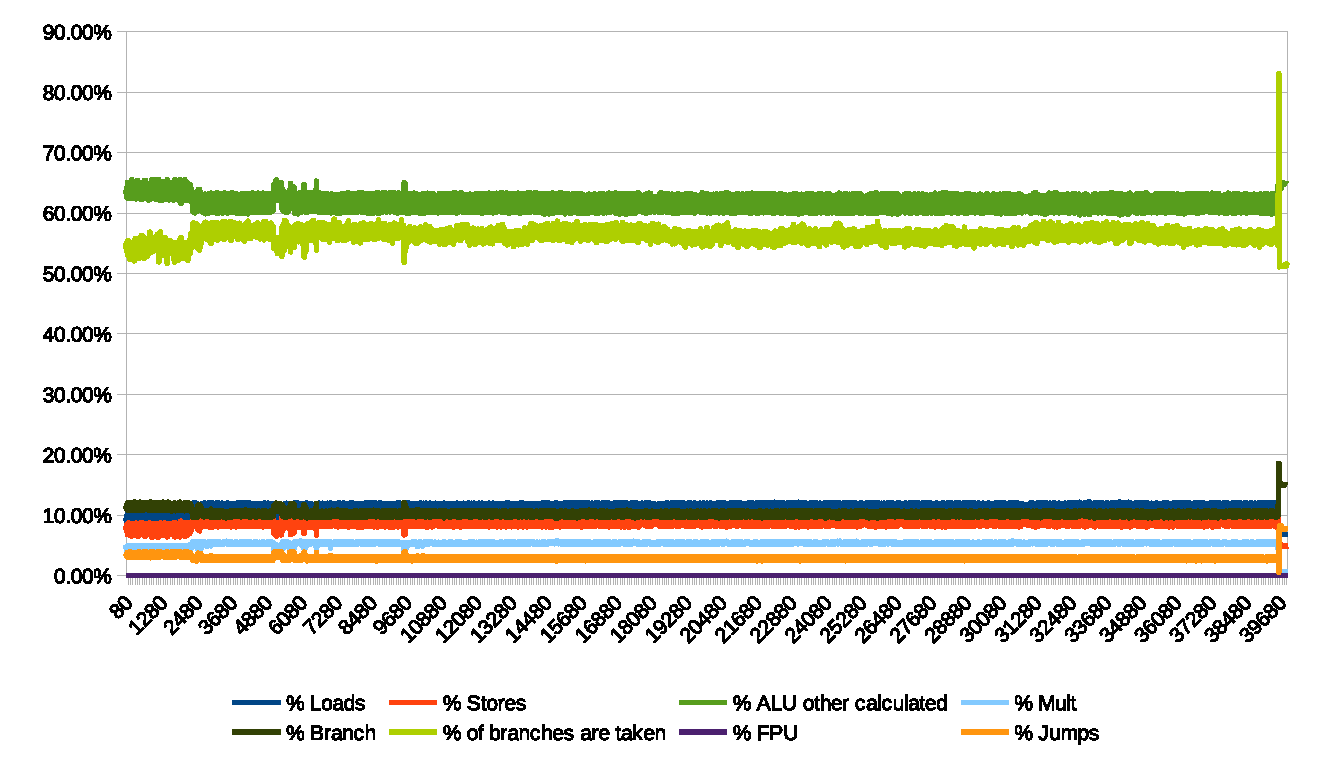
\includegraphics[width=\textwidth]{img/graph/mibench/basicmath_inst.eps}
        \caption{Instruction behavior over time (ms)}
    \end{subfigure}
    \begin{subfigure}{0.45\textwidth}
        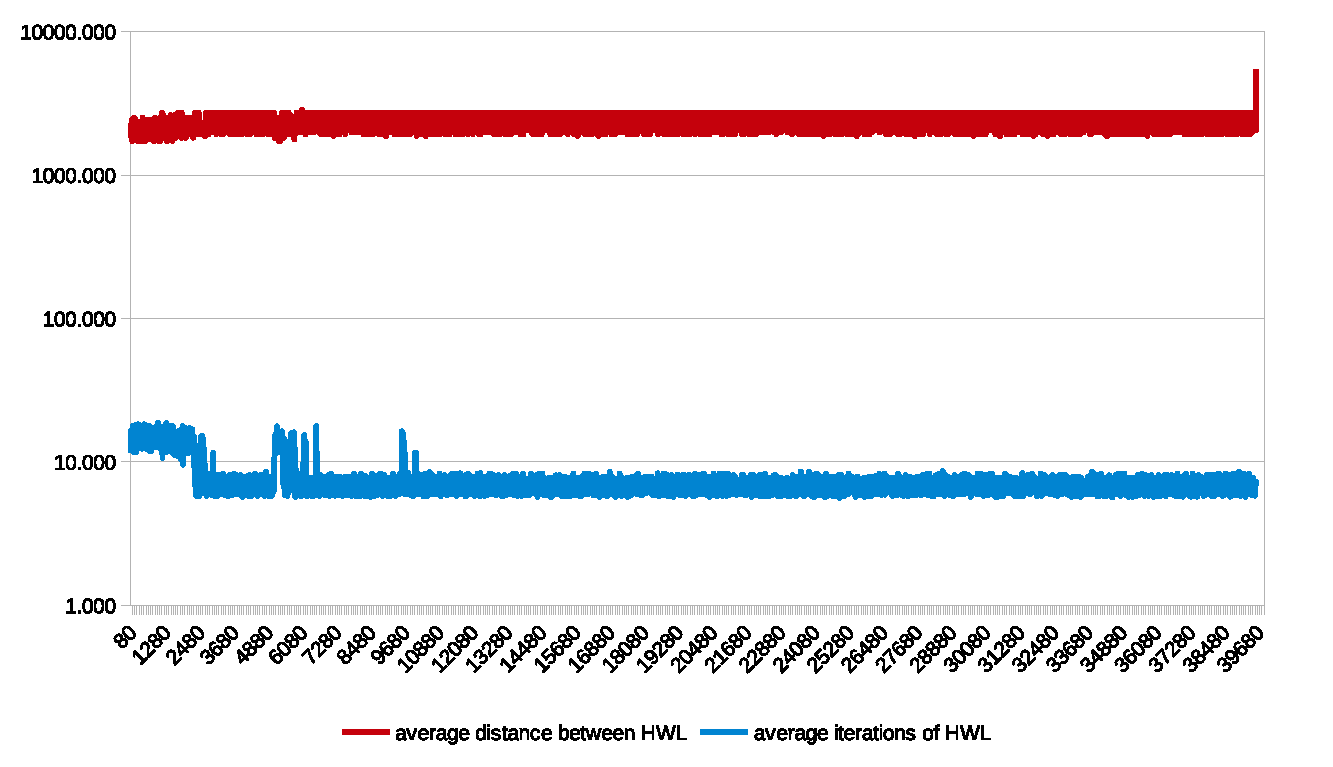
\includegraphics[width=\textwidth]{img/graph/mibench/basicmath_hwl.eps}
        \caption{\ac{HWL} behavior over time (ms)}
    \end{subfigure}
    \begin{subfigure}{0.45\textwidth}
        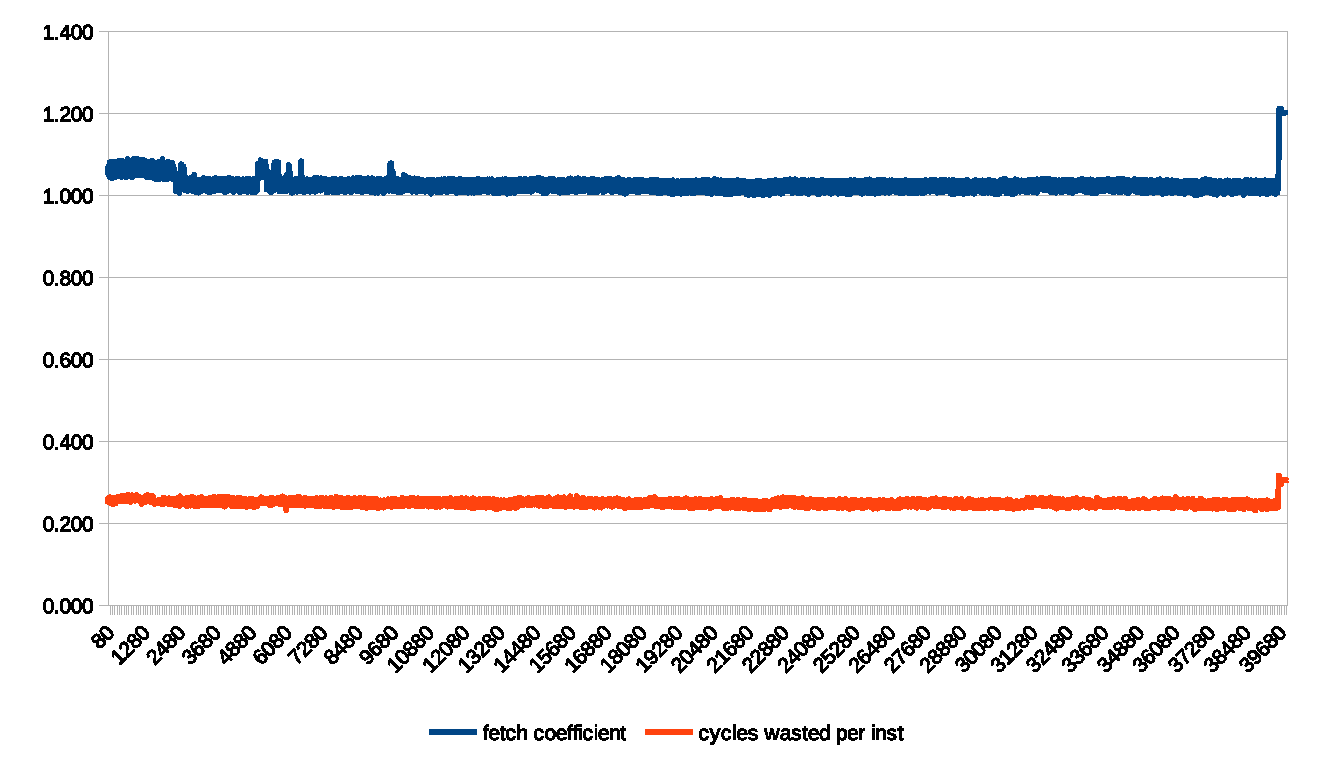
\includegraphics[width=\textwidth]{img/graph/mibench/basicmath_fetch_waste.eps}
        \caption{Fetch coefficient and cycles wasted per instruction over time (ms)}
    \end{subfigure}
    \caption{Performance over time: \texttt{basicmath}}
\end{figure}

% bitcount   
\begin{figure}
    \begin{subfigure}{0.45\textwidth}
        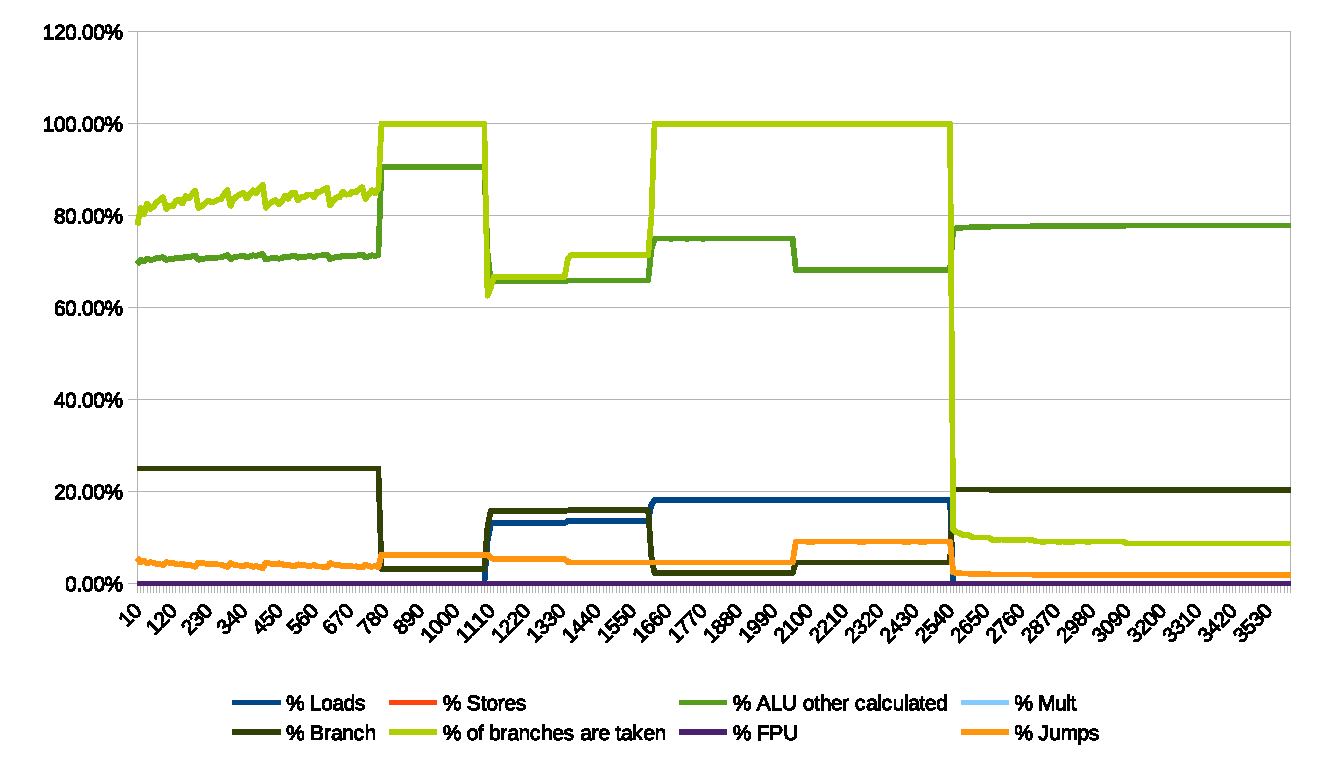
\includegraphics[width=\textwidth]{img/graph/mibench/bitcount_inst.eps}
        \caption{Instruction behavior over time (ms)}
    \end{subfigure}
    \begin{subfigure}{0.45\textwidth}
        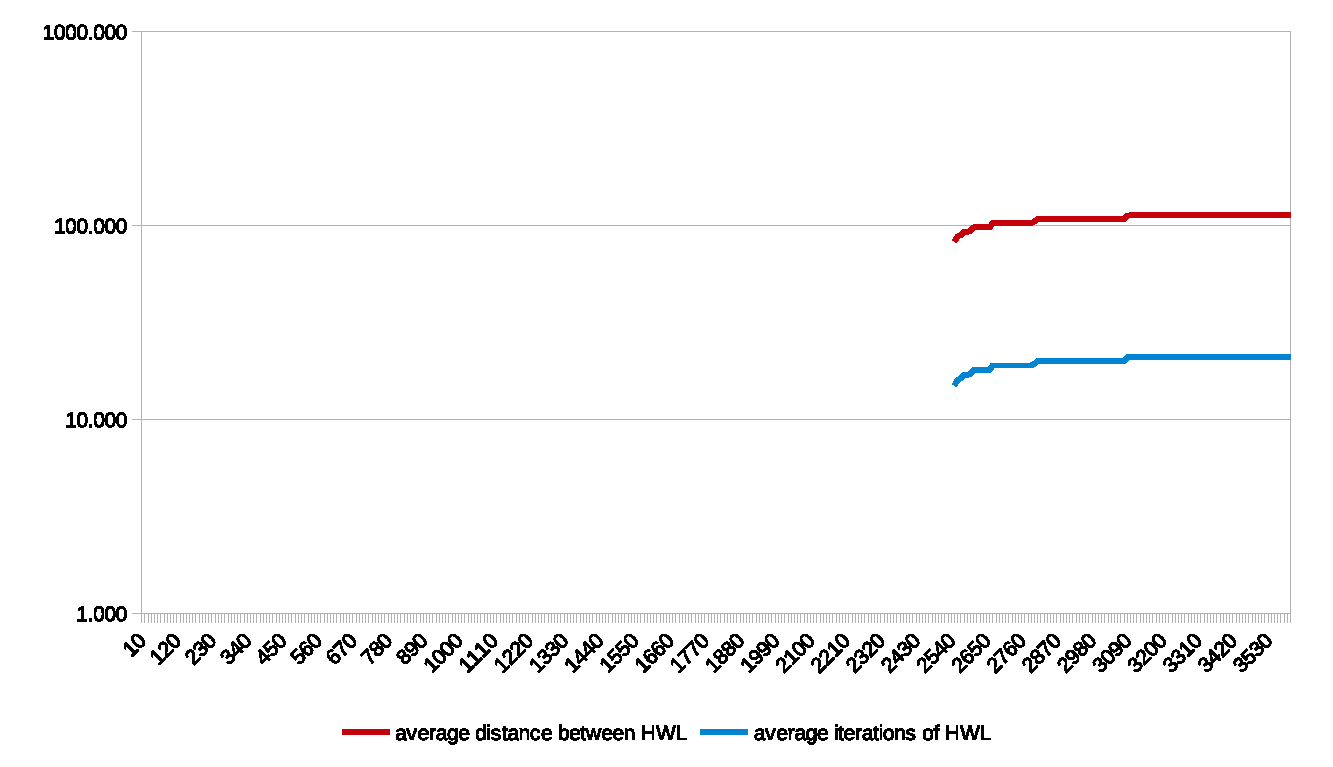
\includegraphics[width=\textwidth]{img/graph/mibench/bitcount_hwl.eps}
        \caption{\ac{HWL} behavior over time (ms)}
    \end{subfigure}
    \begin{subfigure}{0.45\textwidth}
        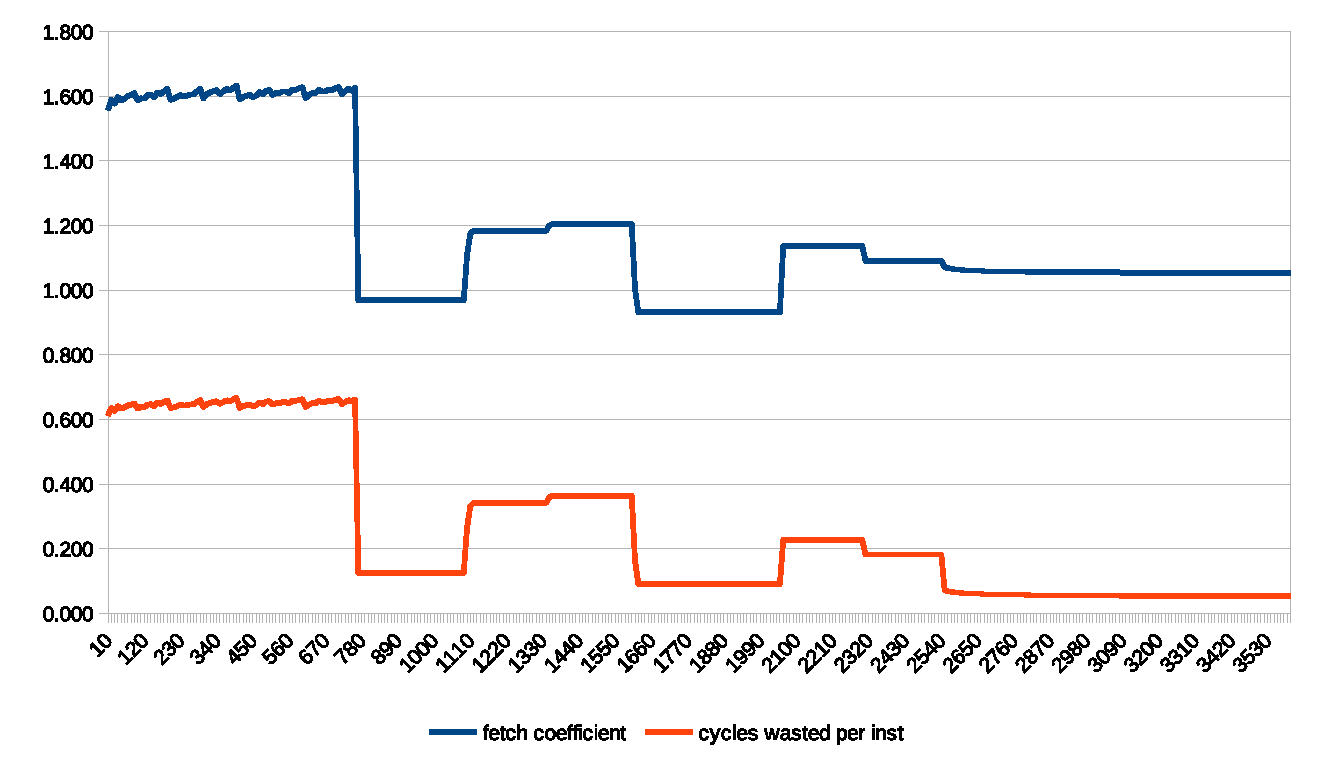
\includegraphics[width=\textwidth]{img/graph/mibench/bitcount_fetch_waste.eps}
        \caption{Fetch coefficient and cycles wasted per instruction over time (ms)}
    \end{subfigure}
    \caption{Performance over time: \texttt{bitcount}}
\end{figure}

% susan   
\begin{figure}
    \begin{subfigure}{0.45\textwidth}
        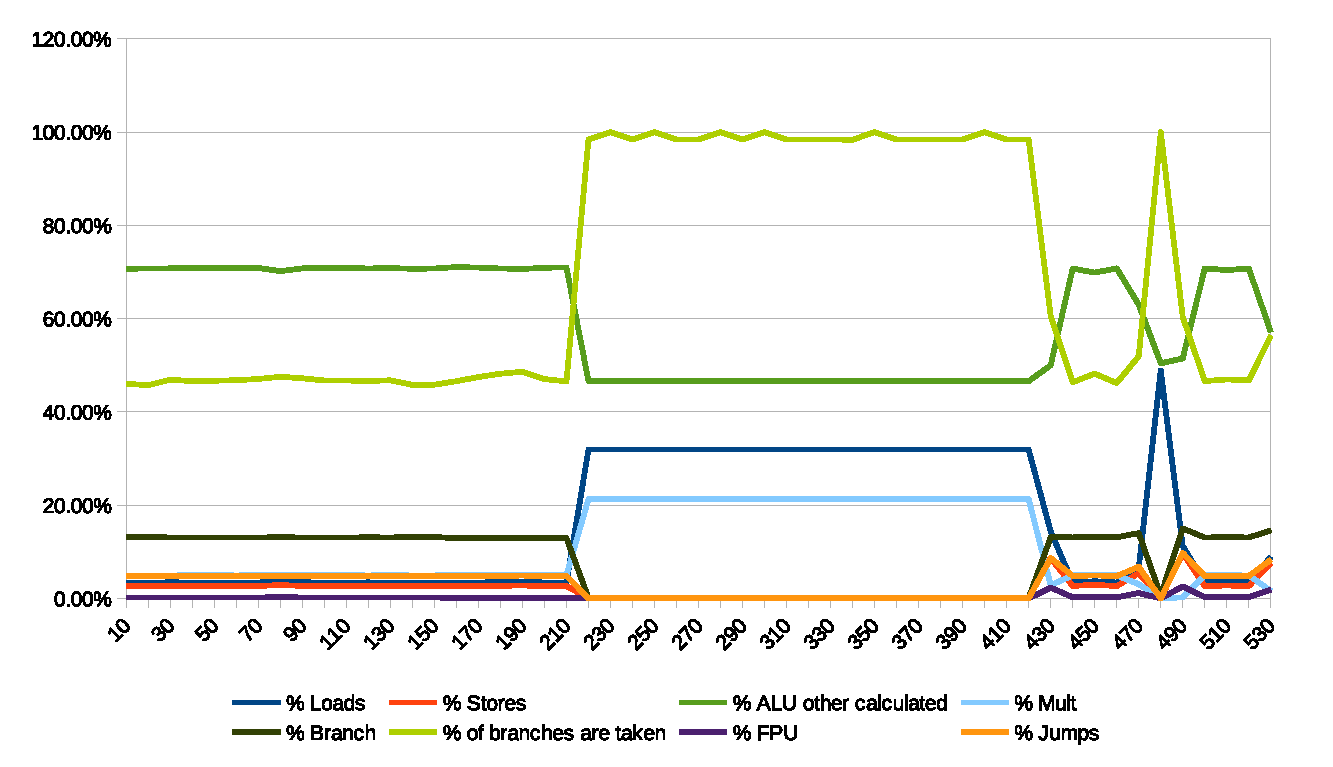
\includegraphics[width=\textwidth]{img/graph/mibench/susan_inst.eps}
        \caption{Instruction behavior over time (ms)}
    \end{subfigure}
    \begin{subfigure}{0.45\textwidth}
        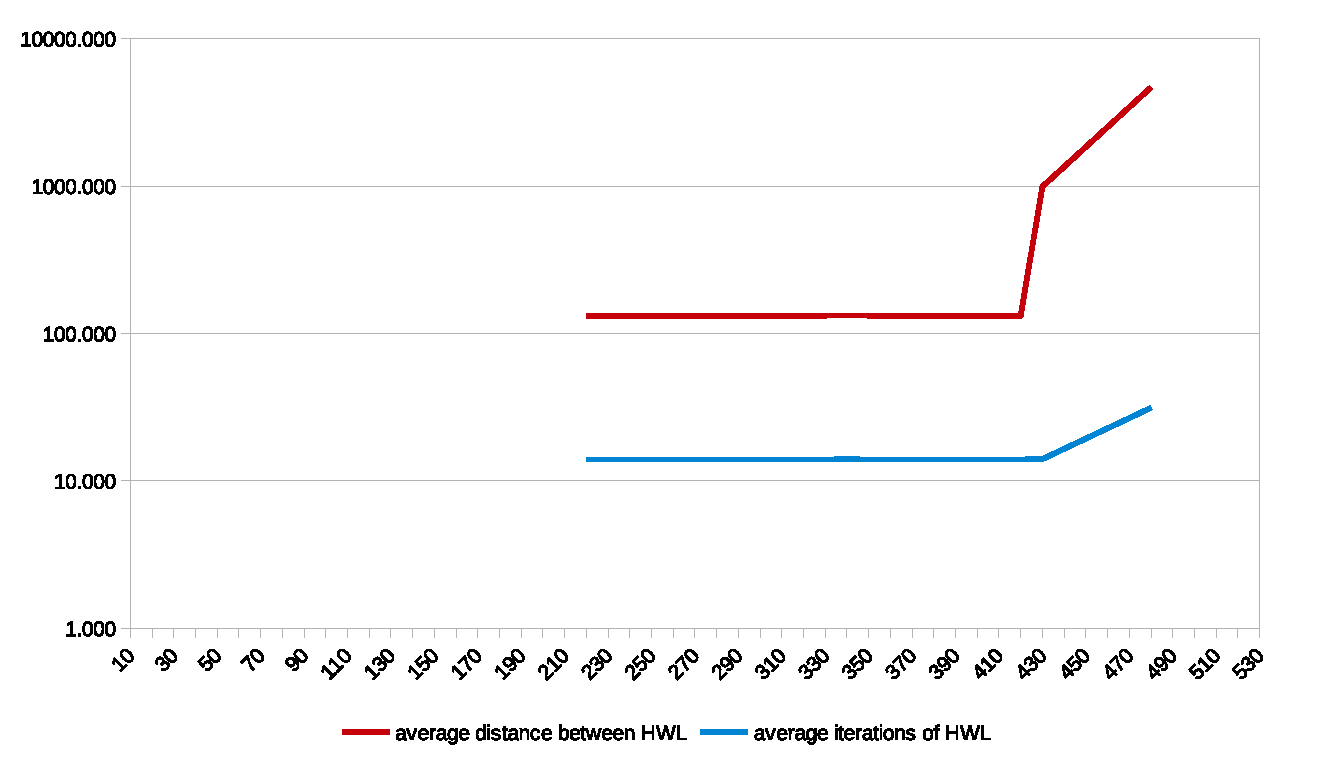
\includegraphics[width=\textwidth]{img/graph/mibench/susan_hwl.eps}
        \caption{\ac{HWL} behavior over time (ms)}
    \end{subfigure}
    \begin{subfigure}{0.45\textwidth}
        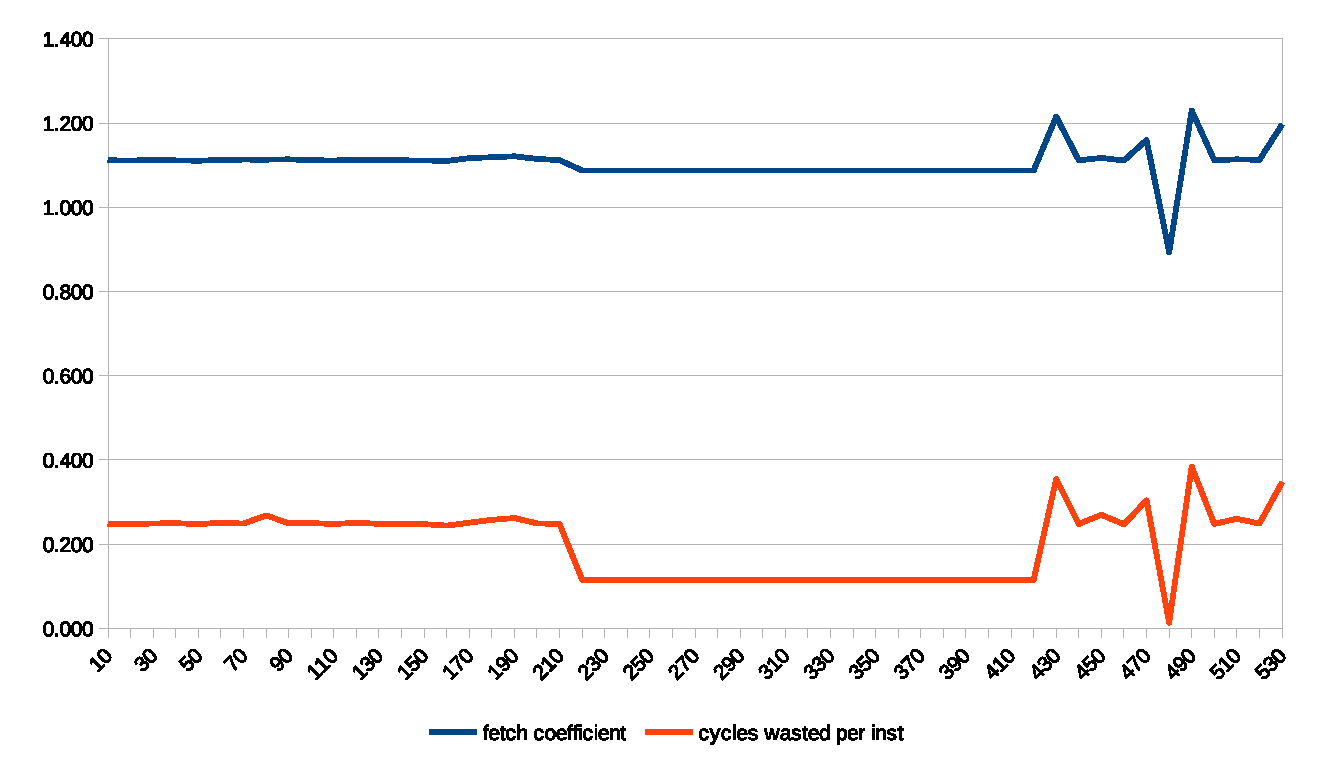
\includegraphics[width=\textwidth]{img/graph/mibench/susan_fetch_waste.eps}
        \caption{Fetch coefficient and cycles wasted per instruction over time (ms)}
    \end{subfigure}
    \caption{Performance over time: \texttt{susan}}
\end{figure}

% dijkstra   
\begin{figure}
    \begin{subfigure}{0.45\textwidth}
        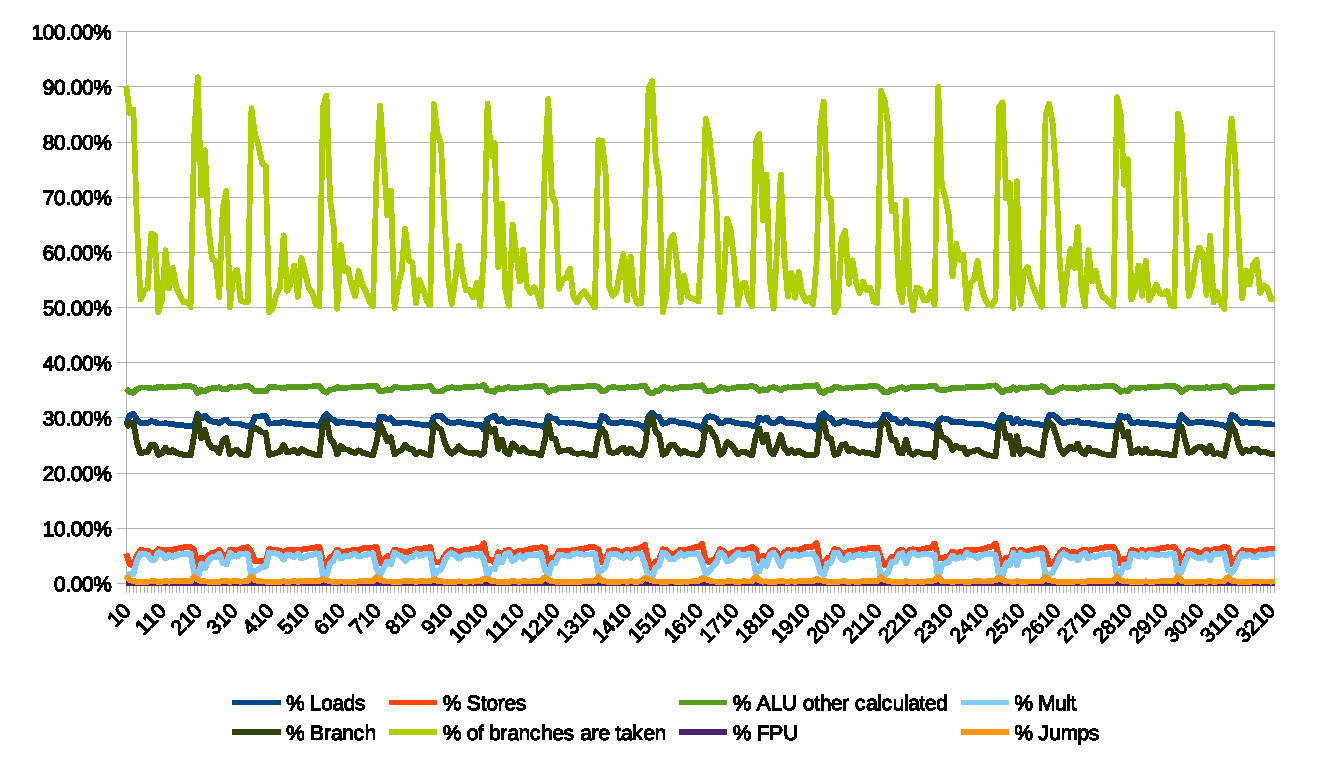
\includegraphics[width=\textwidth]{img/graph/mibench/dijkstra_inst.eps}
        \caption{Instruction behavior over time (ms)}
    \end{subfigure}
    \begin{subfigure}{0.45\textwidth}
        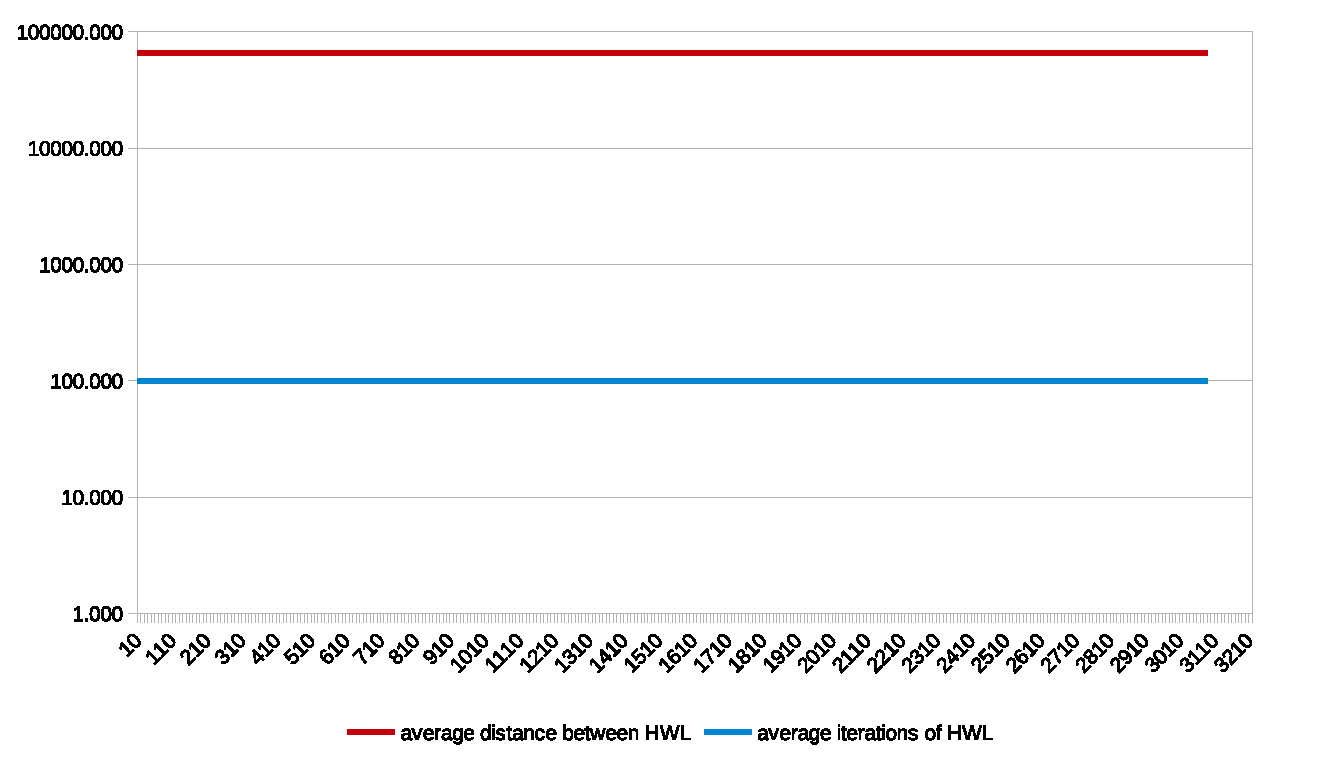
\includegraphics[width=\textwidth]{img/graph/mibench/dijkstra_hwl.eps}
        \caption{\ac{HWL} behavior over time (ms)}
    \end{subfigure}
    \begin{subfigure}{0.45\textwidth}
        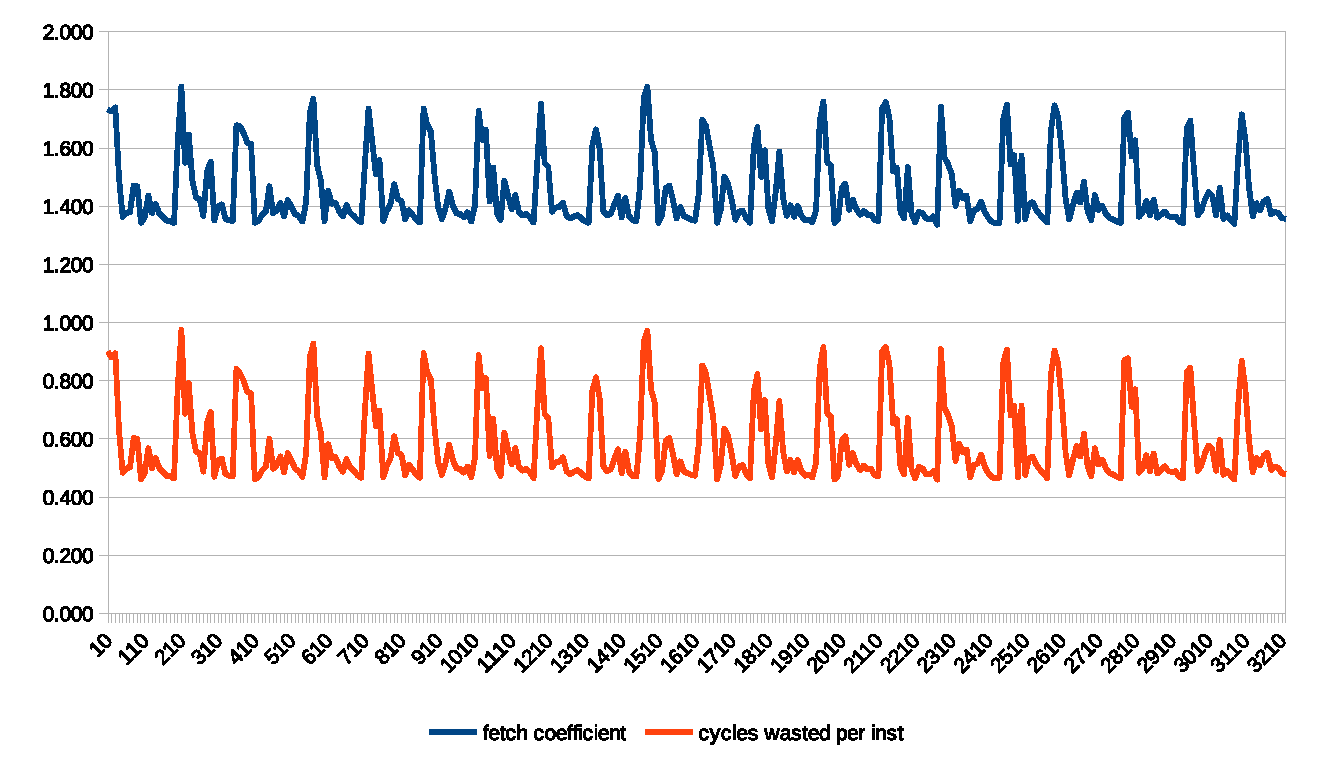
\includegraphics[width=\textwidth]{img/graph/mibench/dijkstra_fetch_waste.eps}
        \caption{Fetch coefficient and cycles wasted per instruction over time (ms)}
    \end{subfigure}
    \caption{Performance over time: \texttt{dijkstra}}
\end{figure}

% fft   
\begin{figure}
    \begin{subfigure}{0.45\textwidth}
        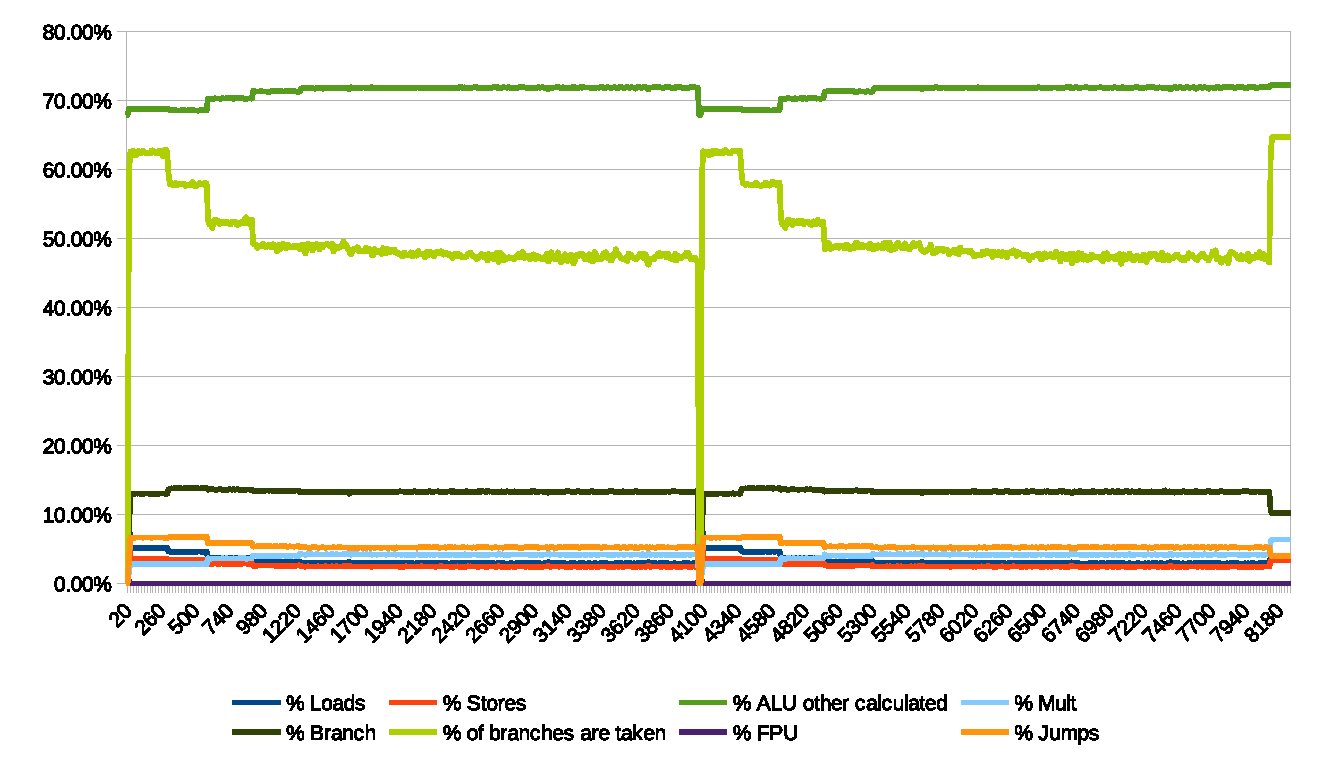
\includegraphics[width=\textwidth]{img/graph/mibench/fft_inst.eps}
        \caption{Instruction behavior over time (ms)}
    \end{subfigure}
    \begin{subfigure}{0.45\textwidth}
        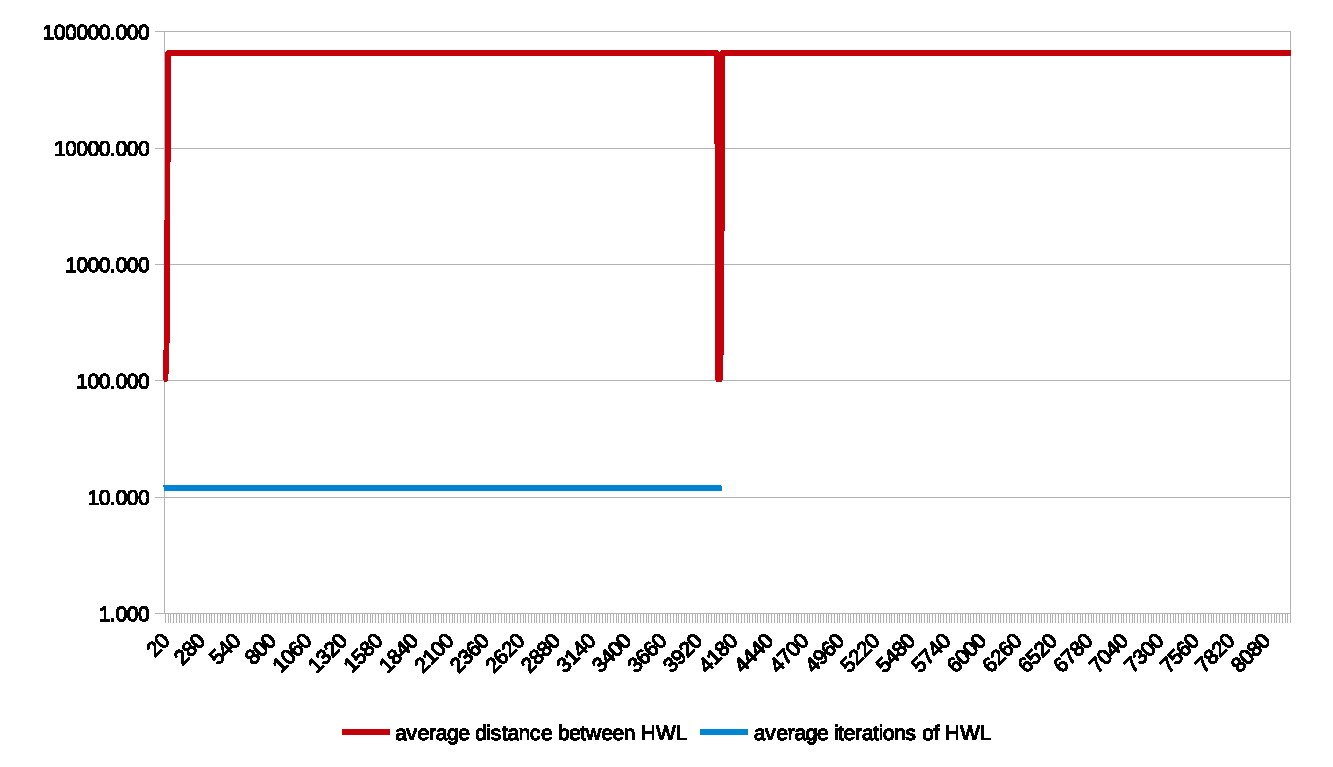
\includegraphics[width=\textwidth]{img/graph/mibench/fft_hwl.eps}
        \caption{\ac{HWL} behavior over time (ms)}
    \end{subfigure}
    \begin{subfigure}{0.45\textwidth}
        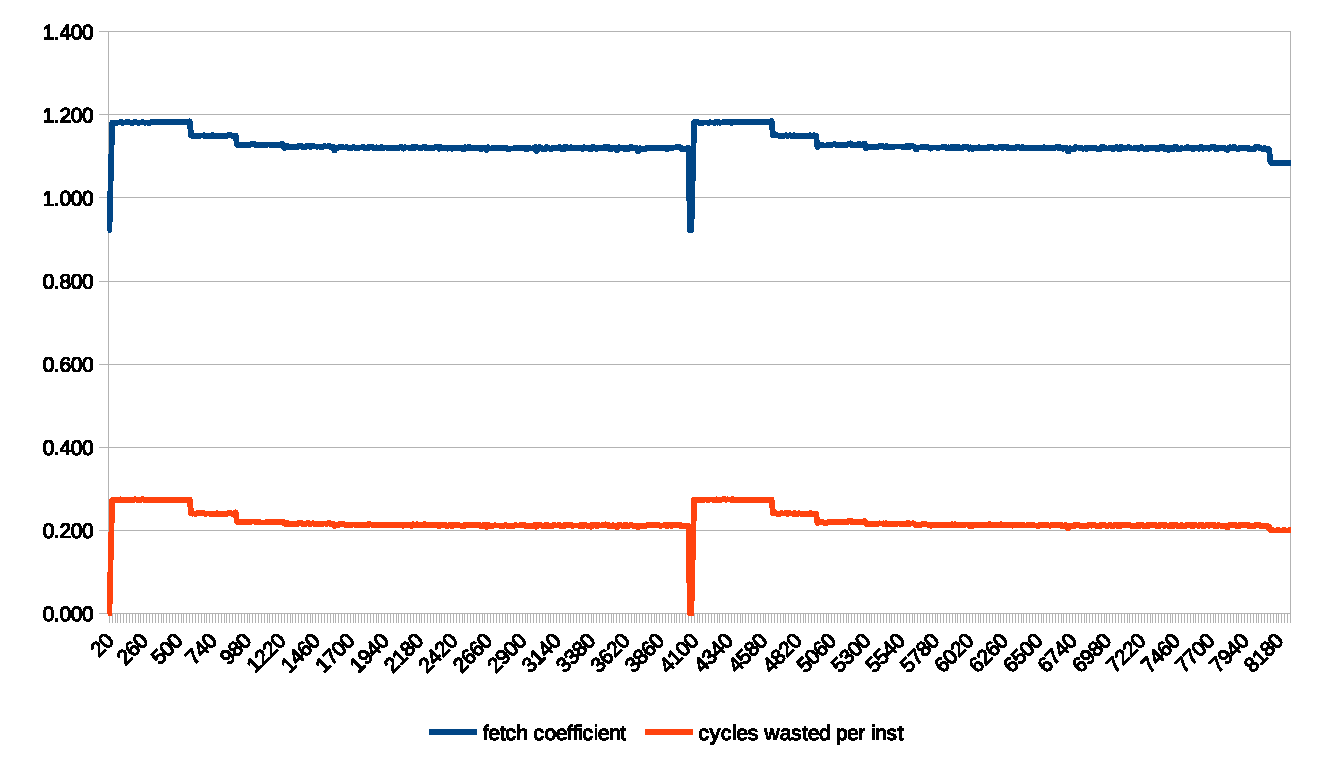
\includegraphics[width=\textwidth]{img/graph/mibench/fft_fetch_waste.eps}
        \caption{Fetch coefficient and cycles wasted per instruction over time (ms)}
    \end{subfigure}
    \caption{Performance over time: \texttt{fft}}
\end{figure}

\FloatBarrier
\section{EmBench}
%%%%%%%%% EMBENCH %%%%%%%%%
% aha-mont64   
\begin{figure}
    \begin{subfigure}{0.45\textwidth}
        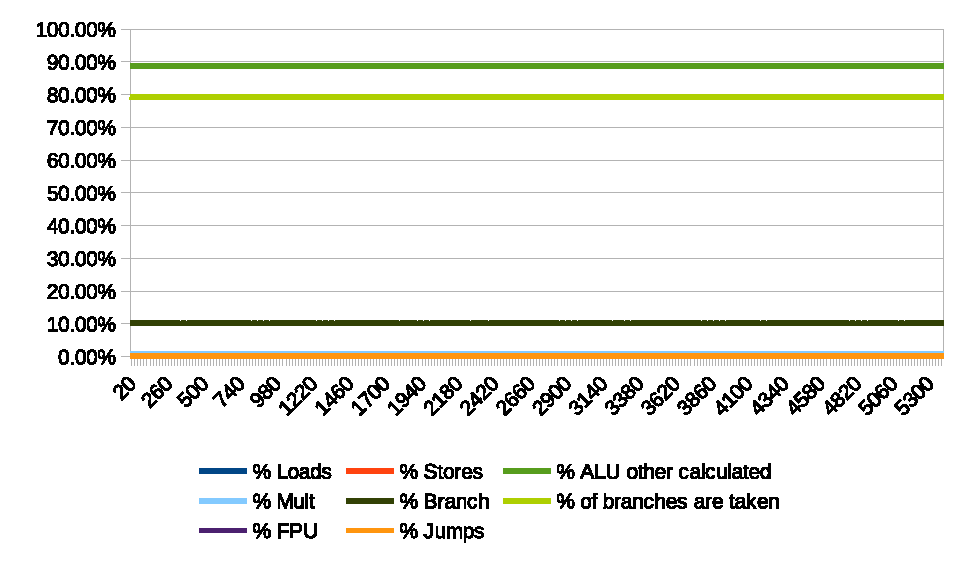
\includegraphics[width=\textwidth]{img/graph/embench/aha-mont64_inst.eps}
        \caption{Instruction behavior over time (ms)}
    \end{subfigure}
    \begin{subfigure}{0.45\textwidth}
        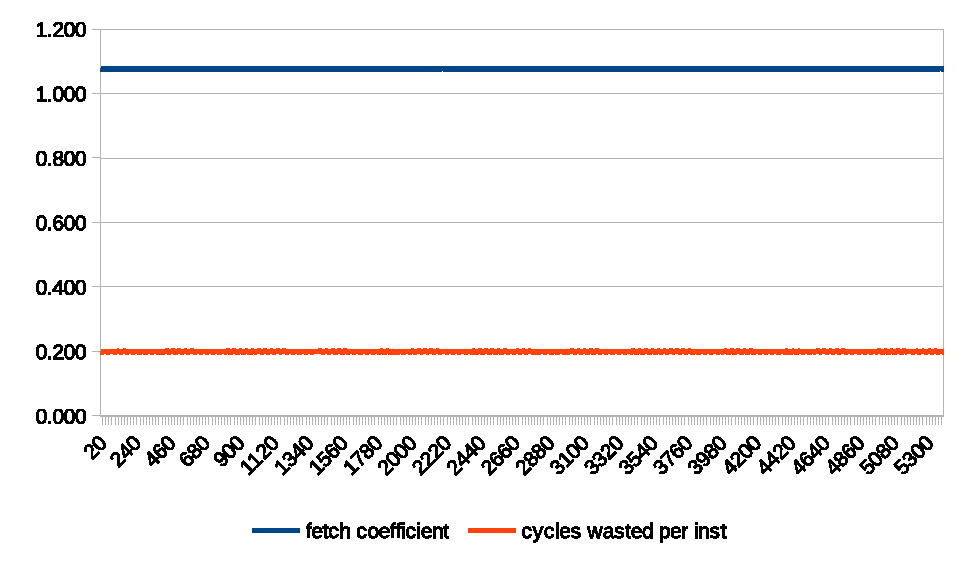
\includegraphics[width=\textwidth]{img/graph/embench/aha-mont64_fetch_waste.eps}
        \caption{Fetch coefficient and cycles wasted per instruction over time (ms)}
    \end{subfigure}
    \caption{Performance over time: \texttt{aha-mont64}}
\end{figure}

% crc32   
\begin{figure}
    \begin{subfigure}{0.45\textwidth}
        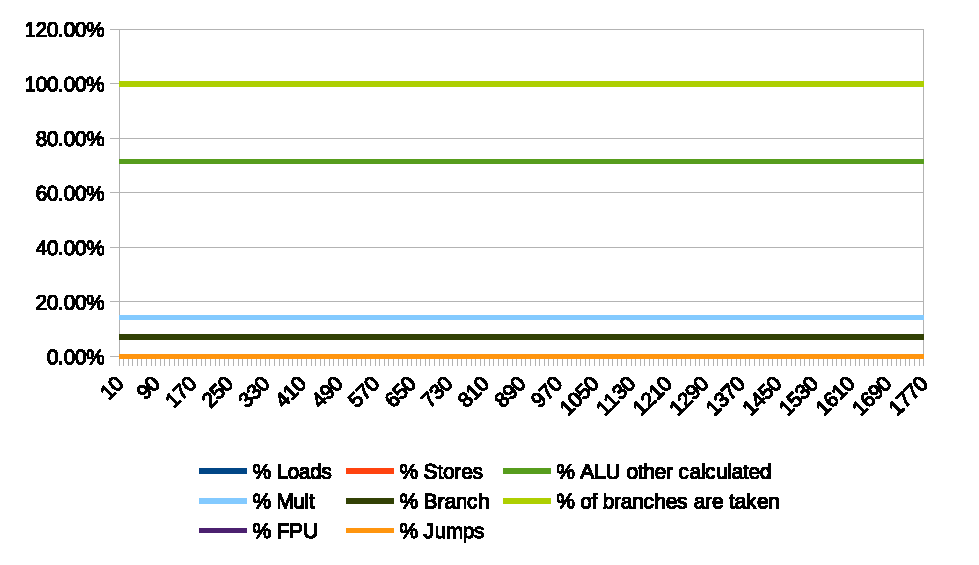
\includegraphics[width=\textwidth]{img/graph/embench/crc32_inst.eps}
        \caption{Instruction behavior over time (ms)}
    \end{subfigure}
    \begin{subfigure}{0.45\textwidth}
        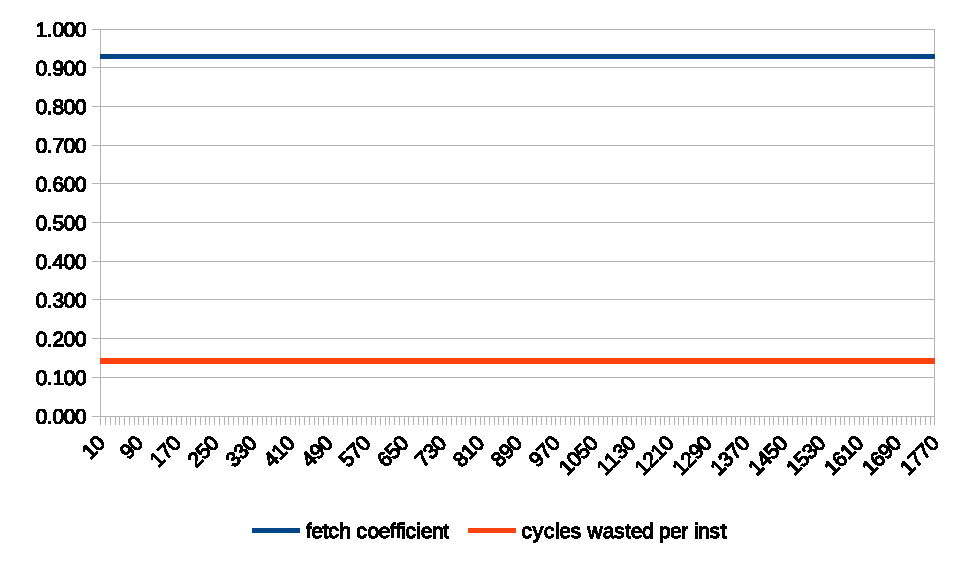
\includegraphics[width=\textwidth]{img/graph/embench/crc32_fetch_waste.eps}
        \caption{Fetch coefficient and cycles wasted per instruction over time (ms)}
    \end{subfigure}
    \caption{Performance over time: \texttt{crc32}}
\end{figure}

% cubic   
\begin{figure}
    \begin{subfigure}{0.45\textwidth}
        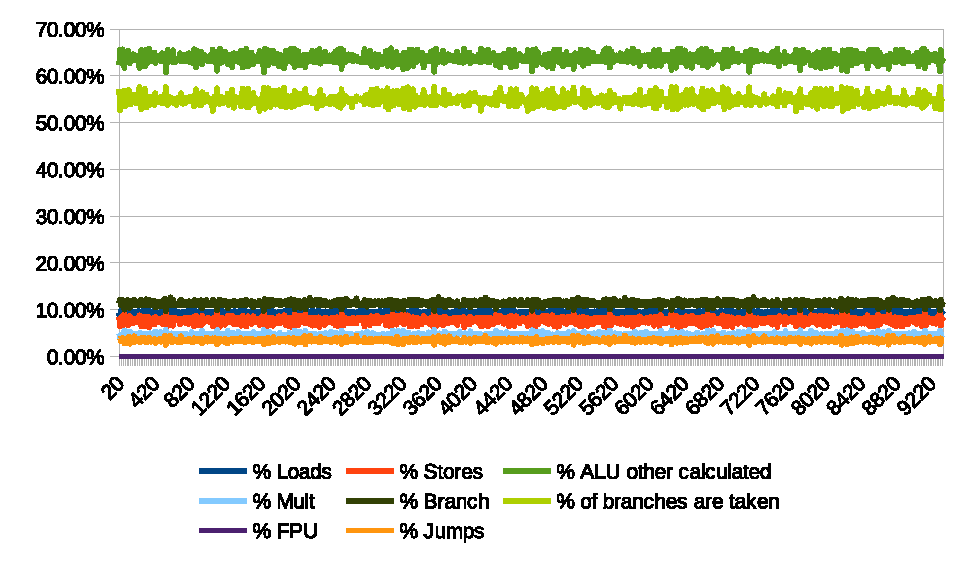
\includegraphics[width=\textwidth]{img/graph/embench/cubic_inst.eps}
        \caption{Instruction behavior over time (ms)}
    \end{subfigure}
    \begin{subfigure}{0.45\textwidth}
        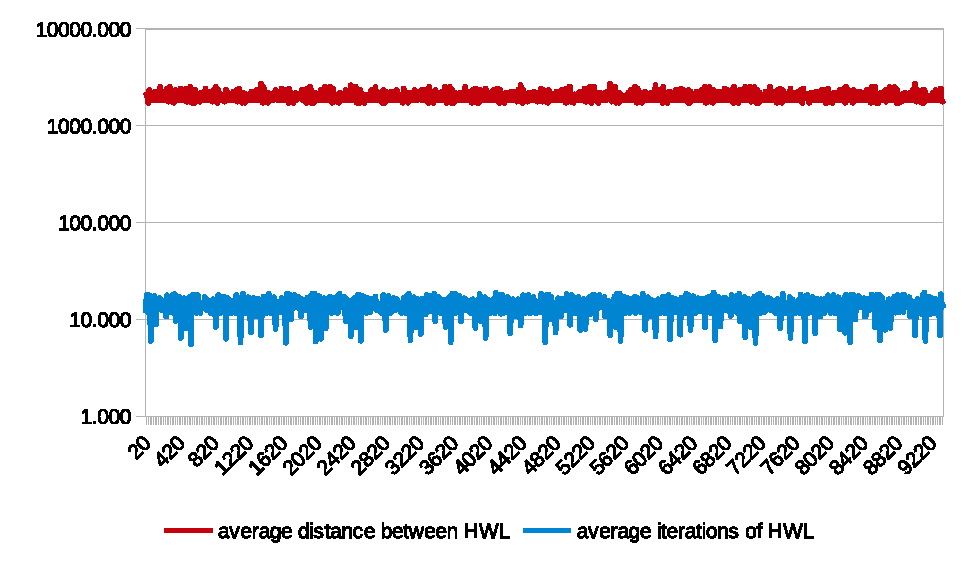
\includegraphics[width=\textwidth]{img/graph/embench/cubic_hwl.eps}
        \caption{\ac{HWL} behavior over time (ms)}
    \end{subfigure}
    \begin{subfigure}{0.45\textwidth}
        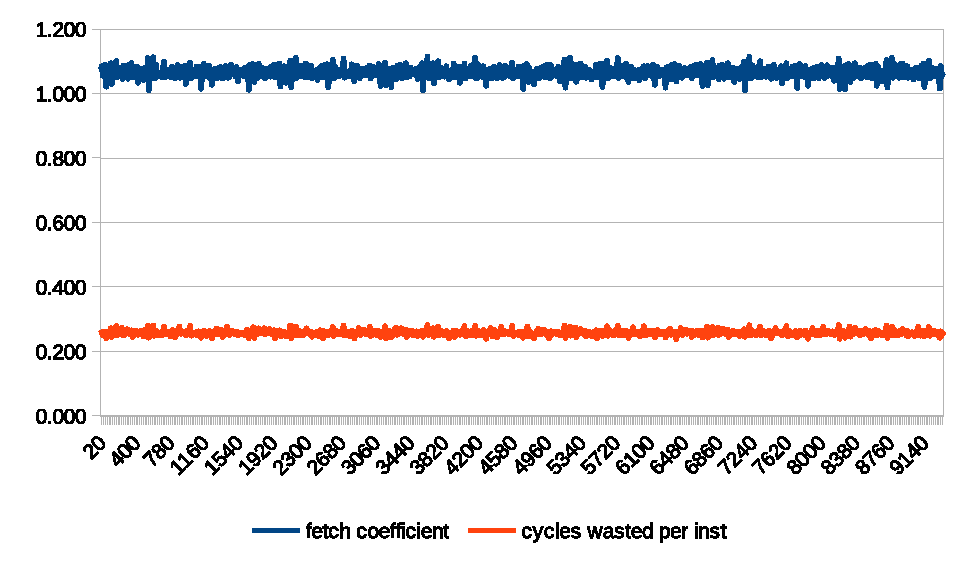
\includegraphics[width=\textwidth]{img/graph/embench/cubic_fetch_waste.eps}
        \caption{Fetch coefficient and cycles wasted per instruction over time (ms)}
    \end{subfigure}
    \caption{Performance over time: \texttt{cubic}}
\end{figure}

% edn   
\begin{figure}
    \begin{subfigure}{0.45\textwidth}
        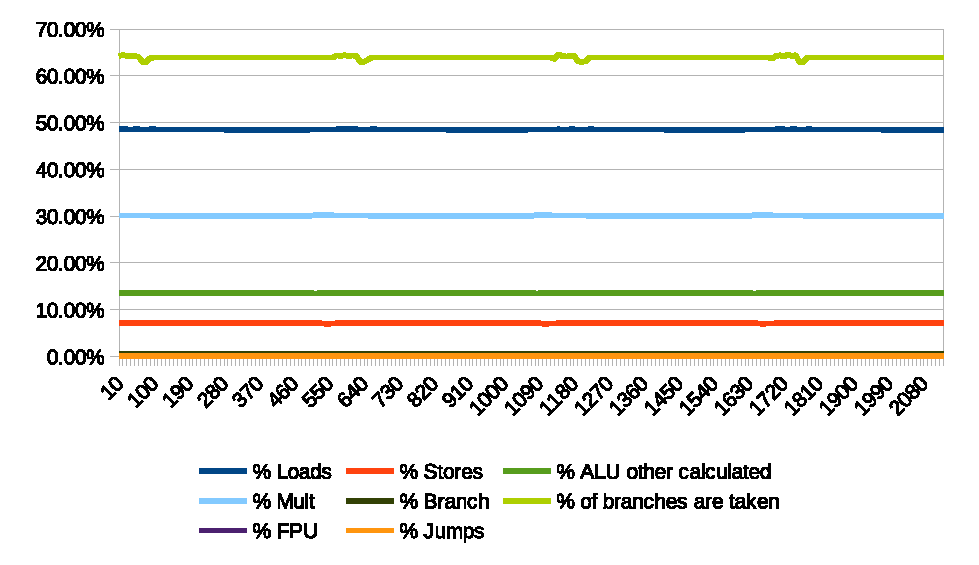
\includegraphics[width=\textwidth]{img/graph/embench/edn_inst.eps}
        \caption{Instruction behavior over time (ms)}
    \end{subfigure}
    \begin{subfigure}{0.45\textwidth}
        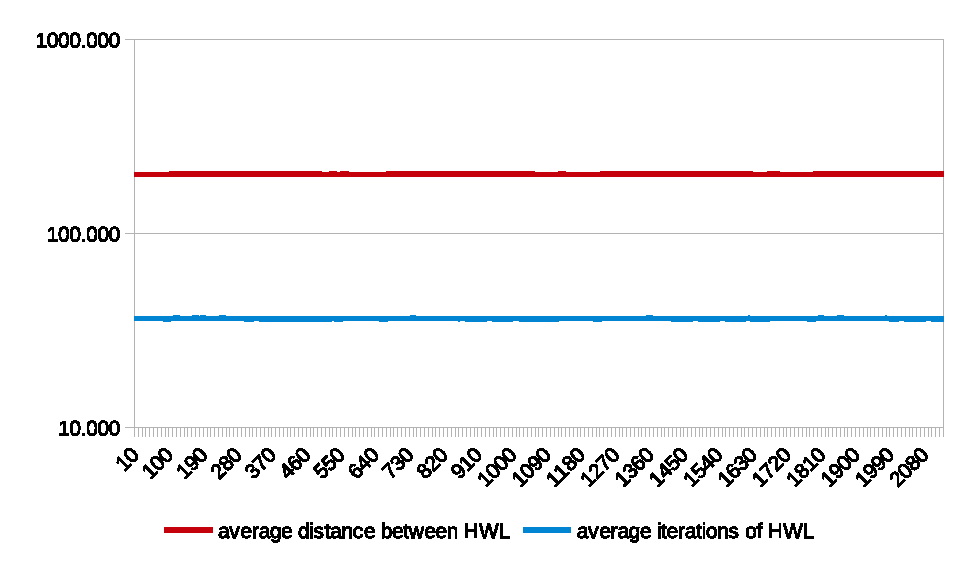
\includegraphics[width=\textwidth]{img/graph/embench/edn_hwl.eps}
        \caption{\ac{HWL} behavior over time (ms)}
    \end{subfigure}
    \begin{subfigure}{0.45\textwidth}
        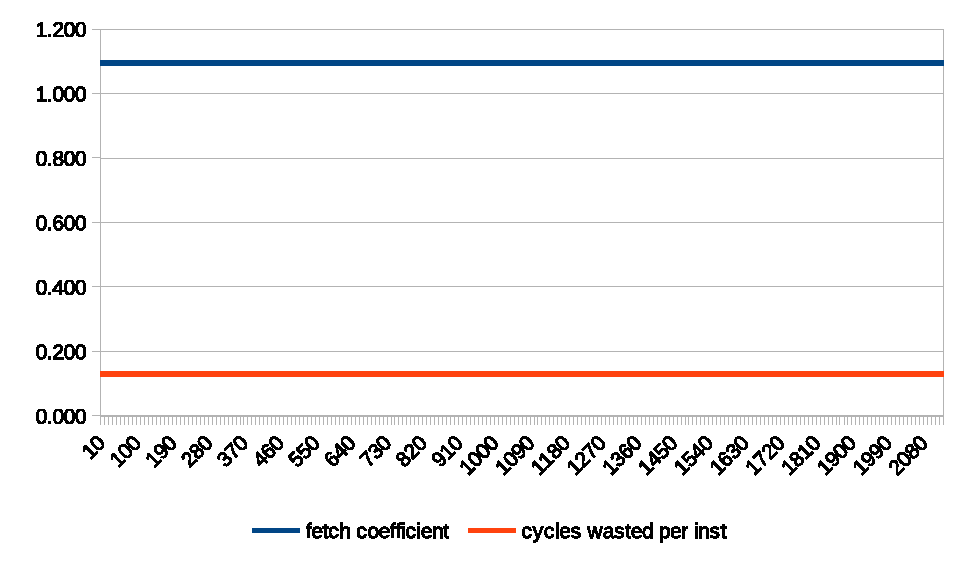
\includegraphics[width=\textwidth]{img/graph/embench/edn_fetch_waste.eps}
        \caption{Fetch coefficient and cycles wasted per instruction over time (ms)}
    \end{subfigure}
    \caption{Performance over time: \texttt{edn}}
\end{figure}

% huffbench   
\begin{figure}
    \begin{subfigure}{0.45\textwidth}
        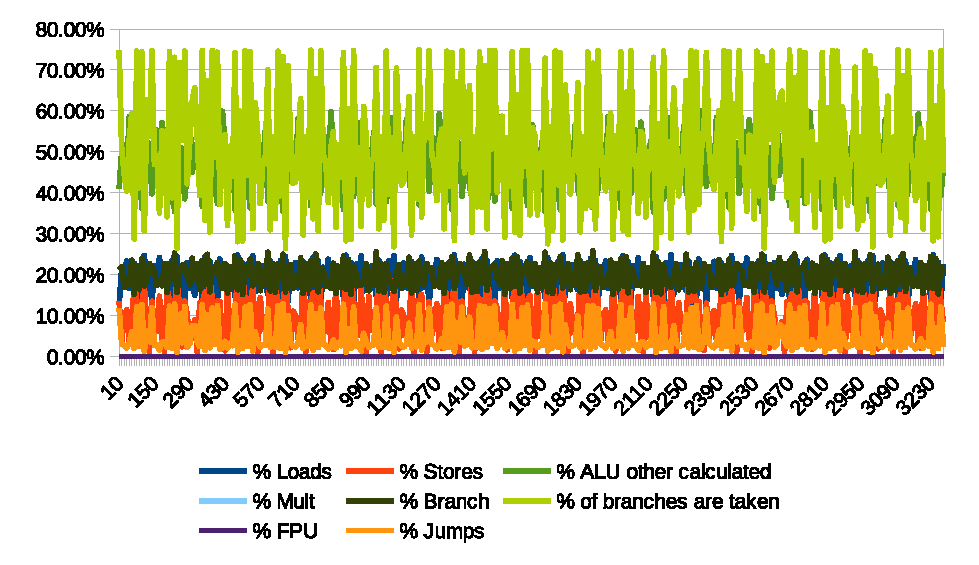
\includegraphics[width=\textwidth]{img/graph/embench/huffbench_inst.eps}
        \caption{Instruction behavior over time (ms)}
    \end{subfigure}
    \begin{subfigure}{0.45\textwidth}
        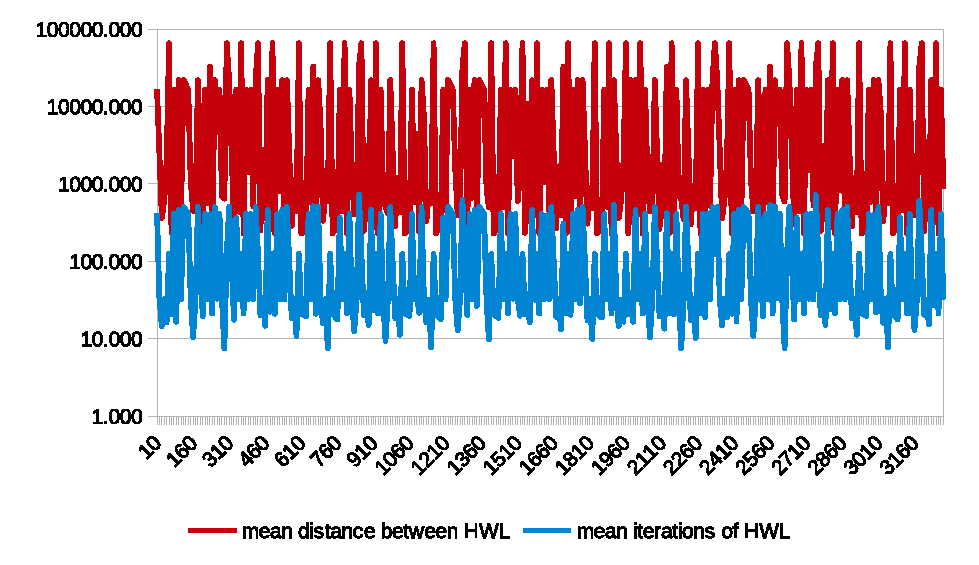
\includegraphics[width=\textwidth]{img/graph/embench/huffbench_hwl.eps}
        \caption{\ac{HWL} behavior over time (ms)}
    \end{subfigure}
    \begin{subfigure}{0.45\textwidth}
        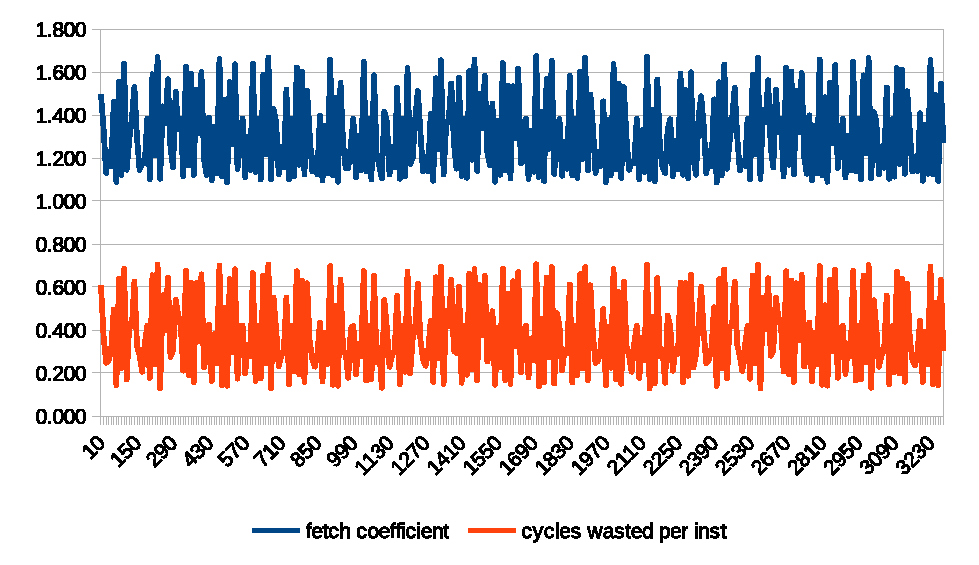
\includegraphics[width=\textwidth]{img/graph/embench/huffbench_fetch_waste.eps}
        \caption{Fetch coefficient and cycles wasted per instruction over time (ms)}
    \end{subfigure}
    \caption{Performance over time: \texttt{huffbench}}
\end{figure}

% matmult-int   
\begin{figure}
    \begin{subfigure}{0.45\textwidth}
        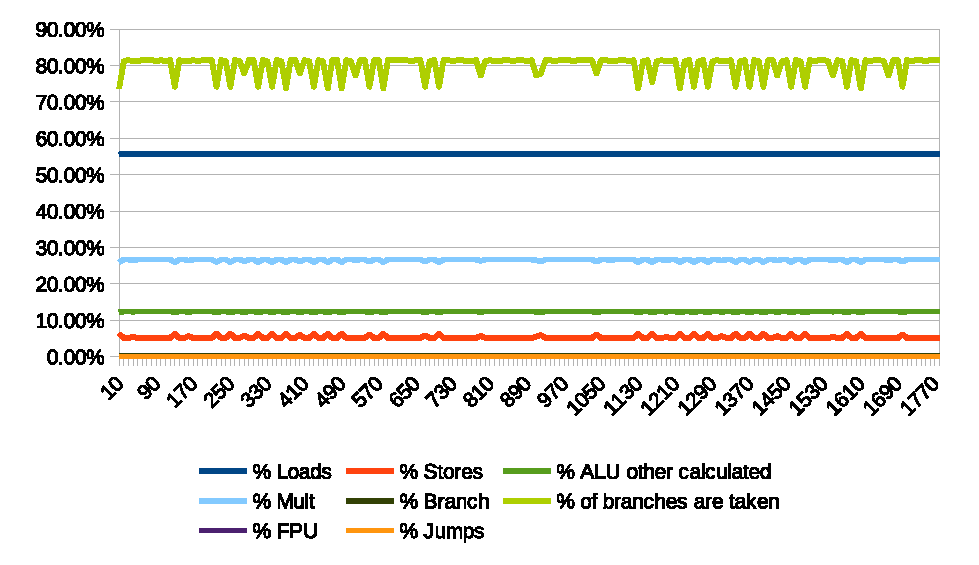
\includegraphics[width=\textwidth]{img/graph/embench/matmult-int_inst.eps}
        \caption{Instruction behavior over time (ms)}
    \end{subfigure}
    \begin{subfigure}{0.45\textwidth}
        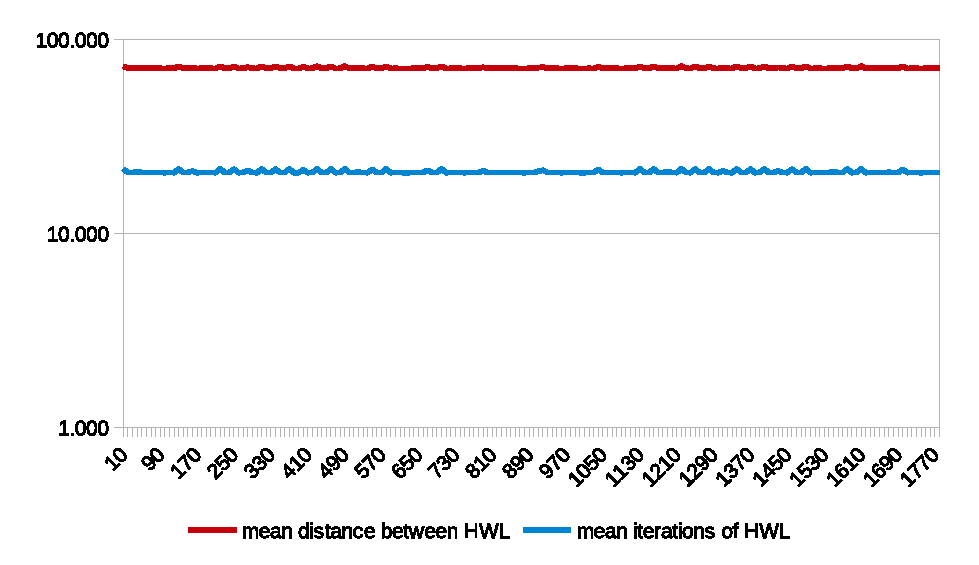
\includegraphics[width=\textwidth]{img/graph/embench/matmult-int_hwl.eps}
        \caption{\ac{HWL} behavior over time (ms)}
    \end{subfigure}
    \begin{subfigure}{0.45\textwidth}
        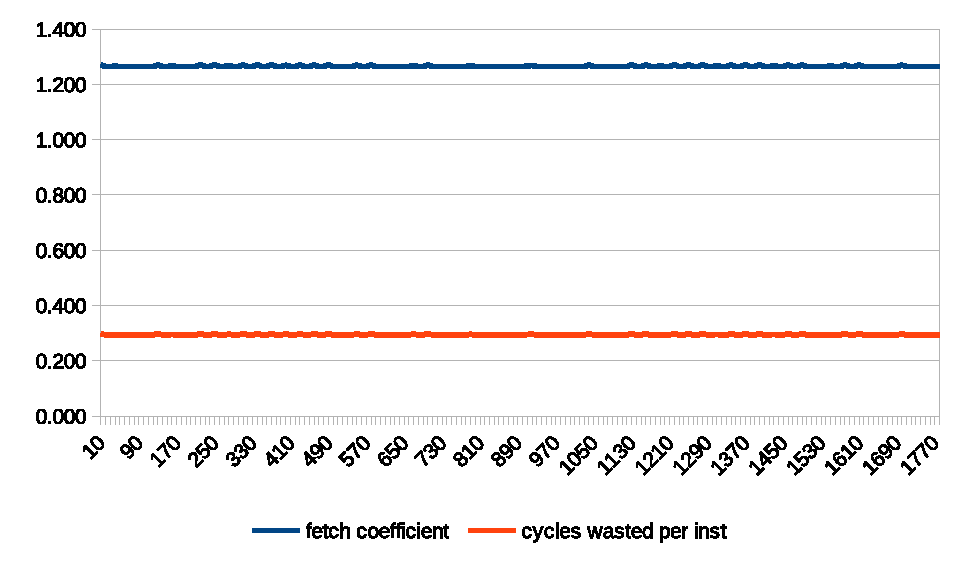
\includegraphics[width=\textwidth]{img/graph/embench/matmult-int_fetch_waste.eps}
        \caption{Fetch coefficient and cycles wasted per instruction over time (ms)}
    \end{subfigure}
    \caption{Performance over time: \texttt{matmult-int}}
\end{figure}

% minver   
\begin{figure}
    \begin{subfigure}{0.45\textwidth}
        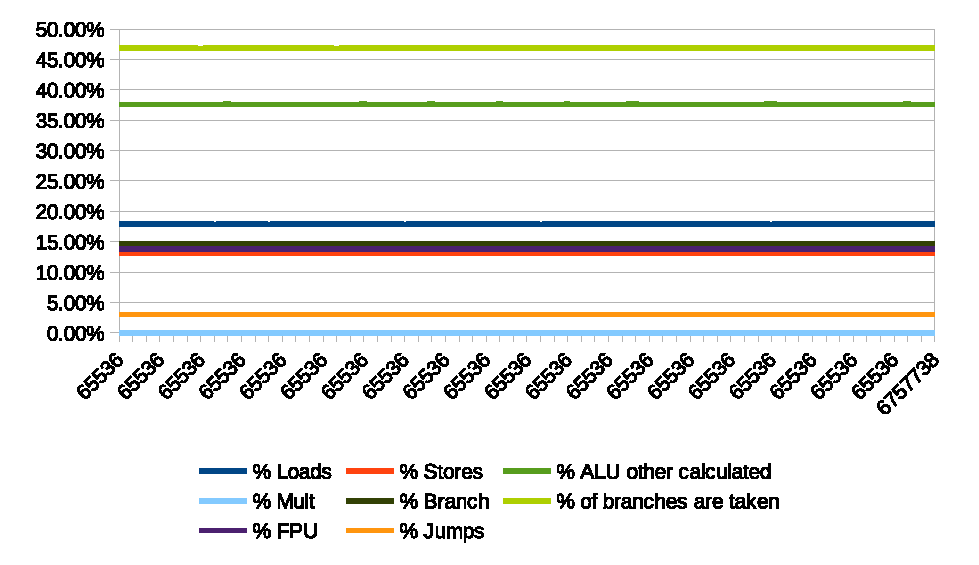
\includegraphics[width=\textwidth]{img/graph/embench/minver_inst.eps}
        \caption{Instruction behavior over time (ms)}
    \end{subfigure}
    \begin{subfigure}{0.45\textwidth}
        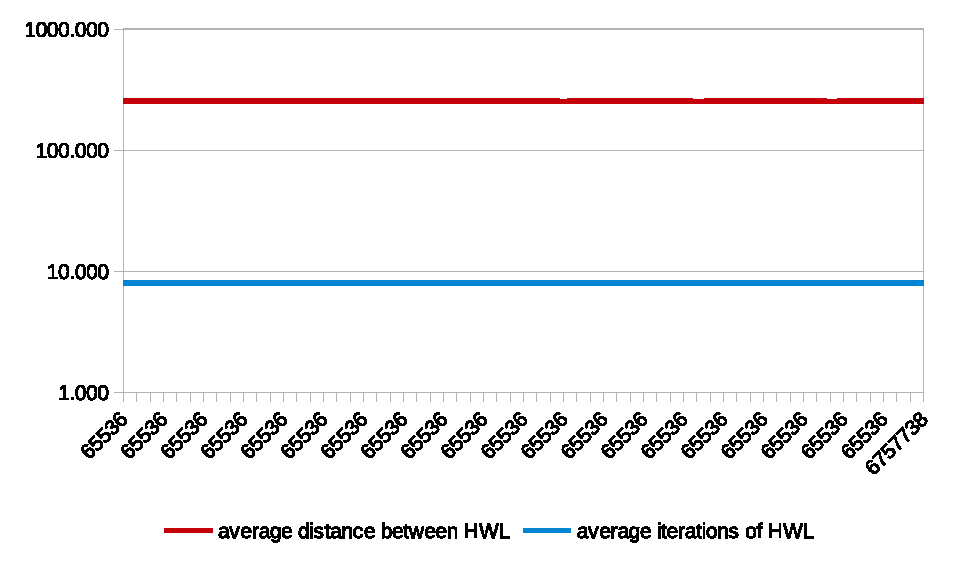
\includegraphics[width=\textwidth]{img/graph/embench/minver_hwl.eps}
        \caption{\ac{HWL} behavior over time (ms)}
    \end{subfigure}
    \begin{subfigure}{0.45\textwidth}
        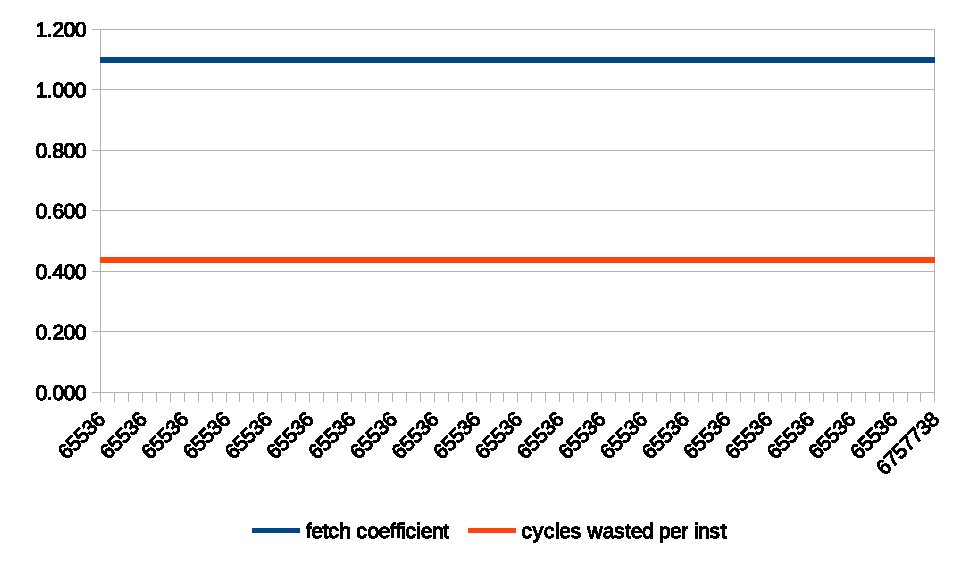
\includegraphics[width=\textwidth]{img/graph/embench/minver_fetch_waste.eps}
        \caption{Fetch coefficient and cycles wasted per instruction over time (ms)}
    \end{subfigure}
    \caption{Performance over time: \texttt{minver}}
\end{figure}

% nbody   
\begin{figure}
    \begin{subfigure}{0.45\textwidth}
        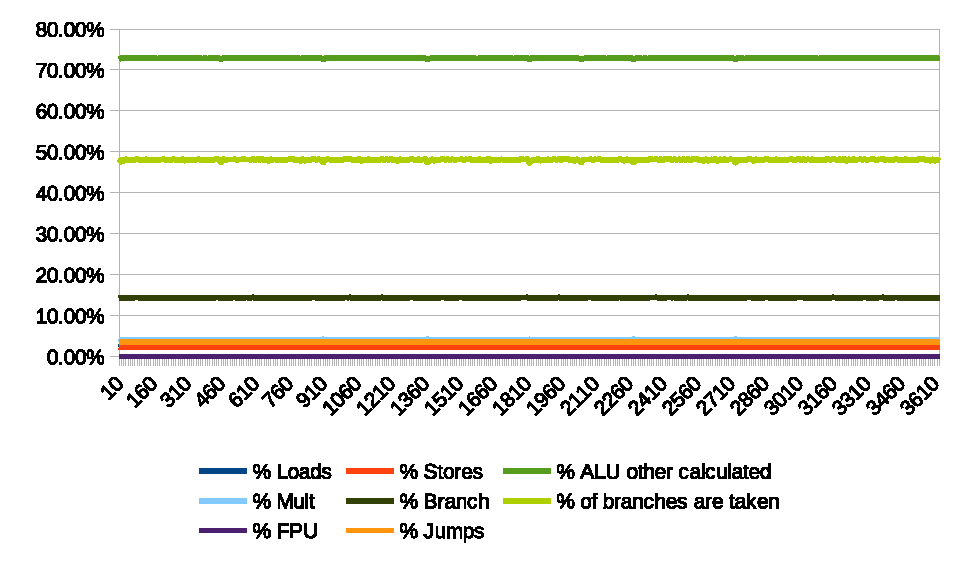
\includegraphics[width=\textwidth]{img/graph/embench/nbody_inst.eps}
        \caption{Instruction behavior over time (ms)}
    \end{subfigure}
    \begin{subfigure}{0.45\textwidth}
        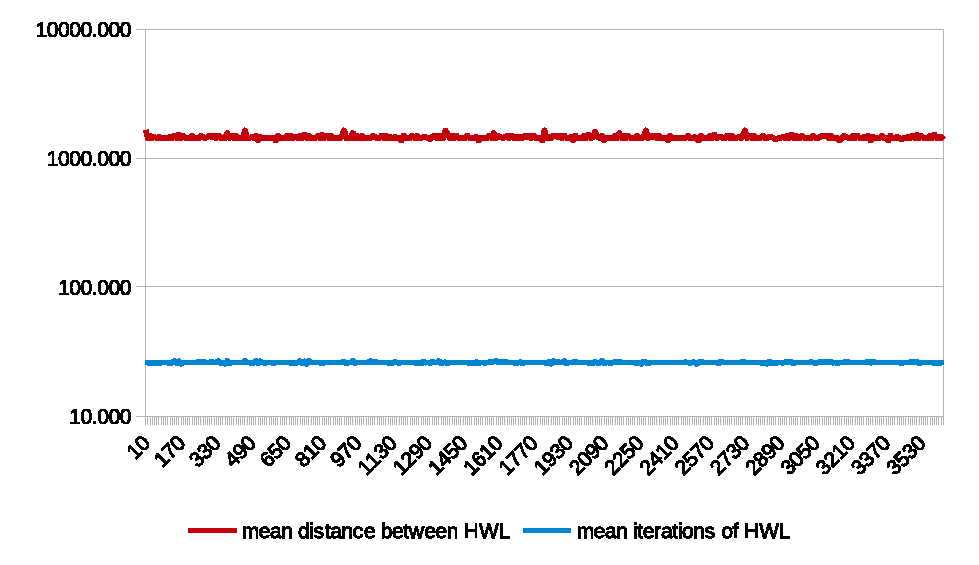
\includegraphics[width=\textwidth]{img/graph/embench/nbody_hwl.eps}
        \caption{\ac{HWL} behavior over time (ms)}
    \end{subfigure}
    \begin{subfigure}{0.45\textwidth}
        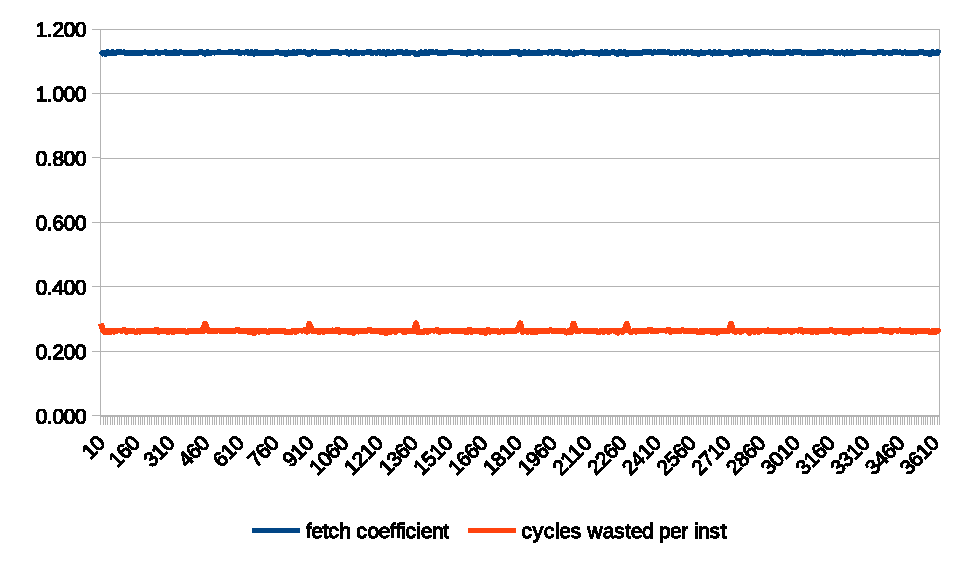
\includegraphics[width=\textwidth]{img/graph/embench/nbody_fetch_waste.eps}
        \caption{Fetch coefficient and cycles wasted per instruction over time (ms)}
    \end{subfigure}
    \caption{Performance over time: \texttt{nbody}}
\end{figure}

% nettle-aes   
\begin{figure}
    \begin{subfigure}{0.45\textwidth}
        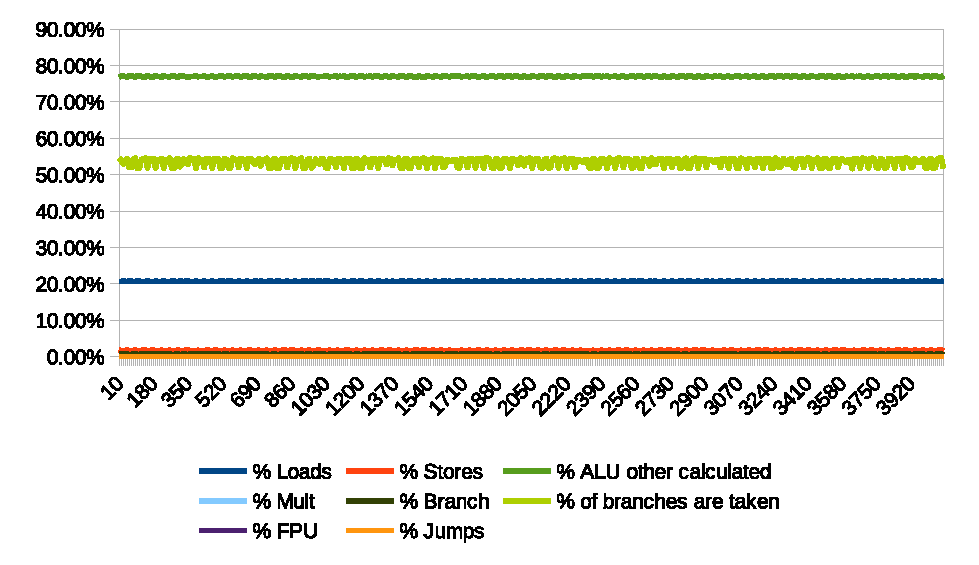
\includegraphics[width=\textwidth]{img/graph/embench/nettle-aes_inst.eps}
        \caption{Instruction behavior over time (ms)}
    \end{subfigure}
    \begin{subfigure}{0.45\textwidth}
        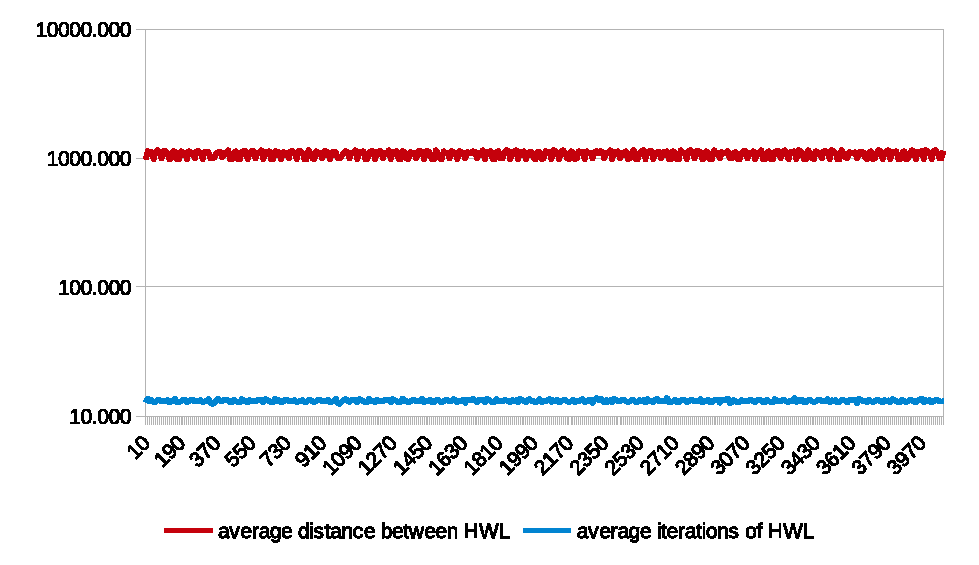
\includegraphics[width=\textwidth]{img/graph/embench/nettle-aes_hwl.eps}
        \caption{\ac{HWL} behavior over time (ms)}
    \end{subfigure}
    \begin{subfigure}{0.45\textwidth}
        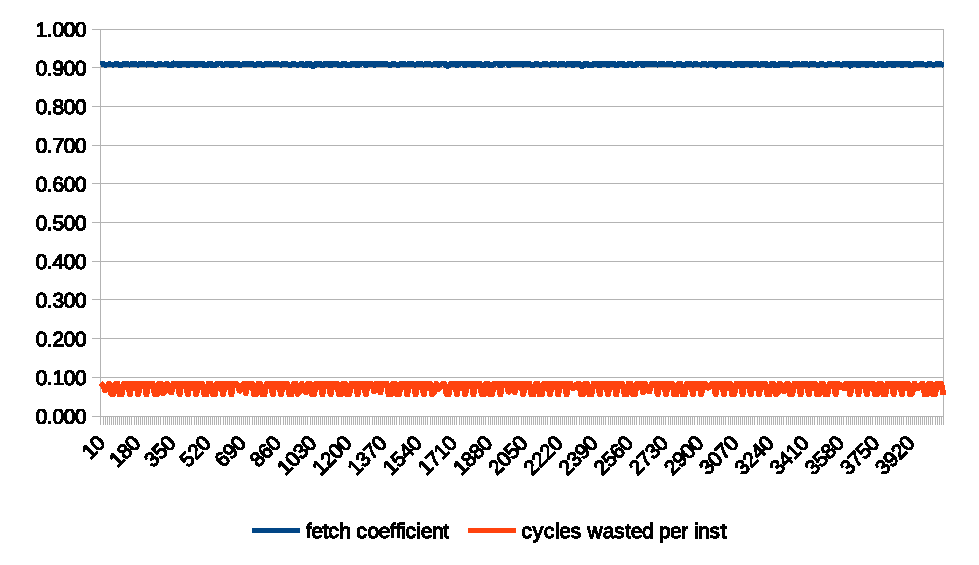
\includegraphics[width=\textwidth]{img/graph/embench/nettle-aes_fetch_waste.eps}
        \caption{Fetch coefficient and cycles wasted per instruction over time (ms)}
    \end{subfigure}
    \caption{Performance over time: \texttt{nettle-aes}}
\end{figure}

% nettle-sha256   
\begin{figure}
    \begin{subfigure}{0.45\textwidth}
        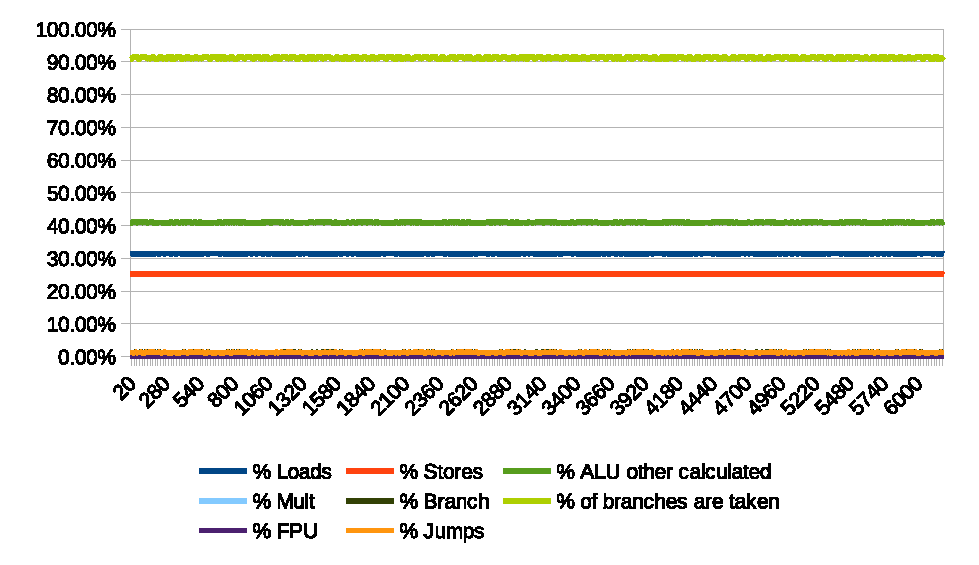
\includegraphics[width=\textwidth]{img/graph/embench/nettle-sha256_inst.eps}
        \caption{Instruction behavior over time (ms)}
    \end{subfigure}
    \begin{subfigure}{0.45\textwidth}
        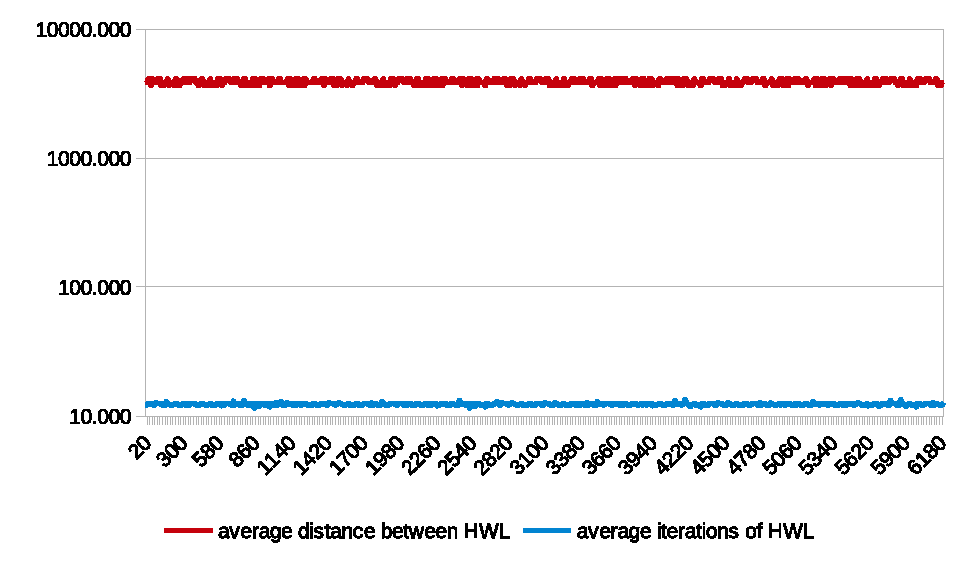
\includegraphics[width=\textwidth]{img/graph/embench/nettle-sha256_hwl.eps}
        \caption{\ac{HWL} behavior over time (ms)}
    \end{subfigure}
    \begin{subfigure}{0.45\textwidth}
        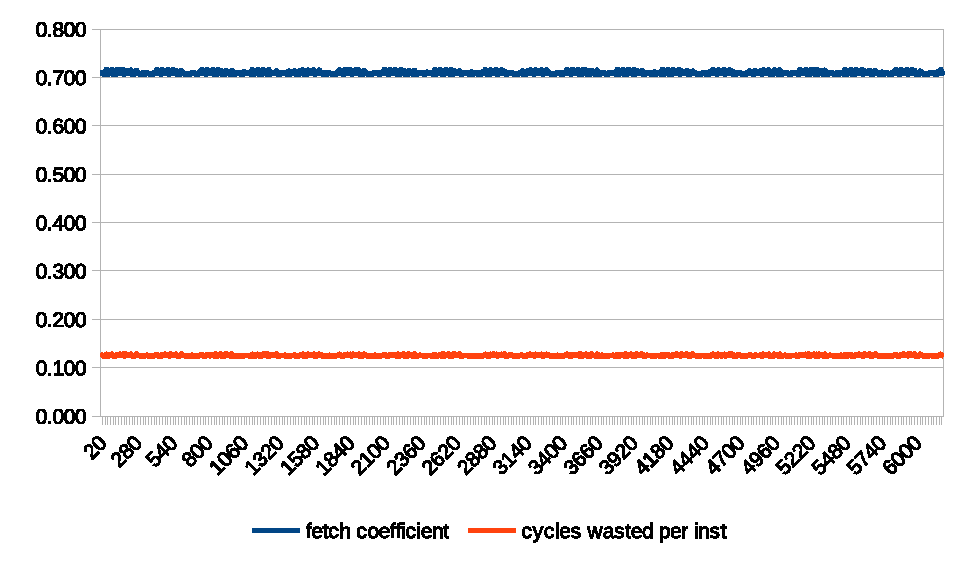
\includegraphics[width=\textwidth]{img/graph/embench/nettle-sha256_fetch_waste.eps}
        \caption{Fetch coefficient and cycles wasted per instruction over time (ms)}
    \end{subfigure}
    \caption{Performance over time: \texttt{nettle-sha256}}
\end{figure}

% nsichneu   
\begin{figure}
    \begin{subfigure}{0.45\textwidth}
        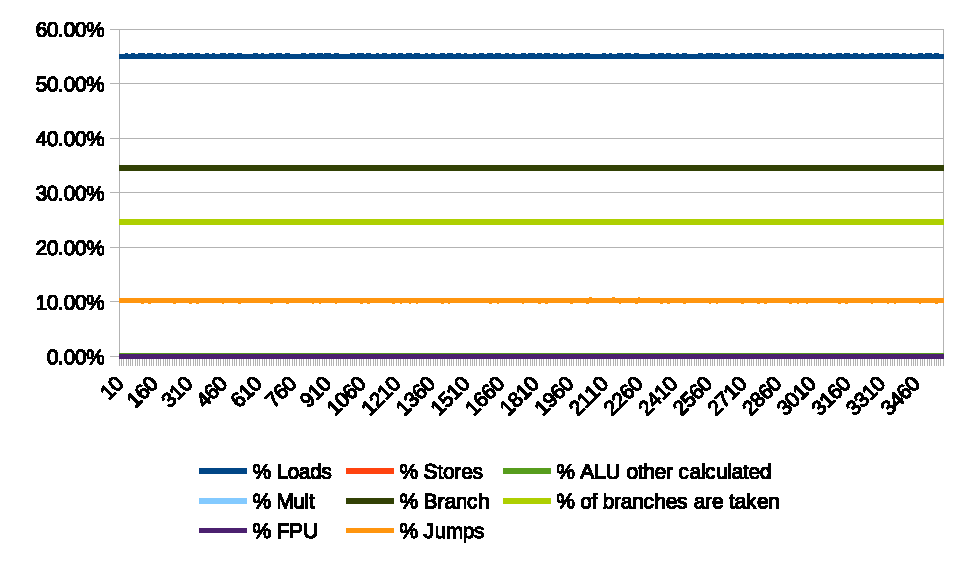
\includegraphics[width=\textwidth]{img/graph/embench/nsichneu_inst.eps}
        \caption{Instruction behavior over time (ms)}
    \end{subfigure}
    \begin{subfigure}{0.45\textwidth}
        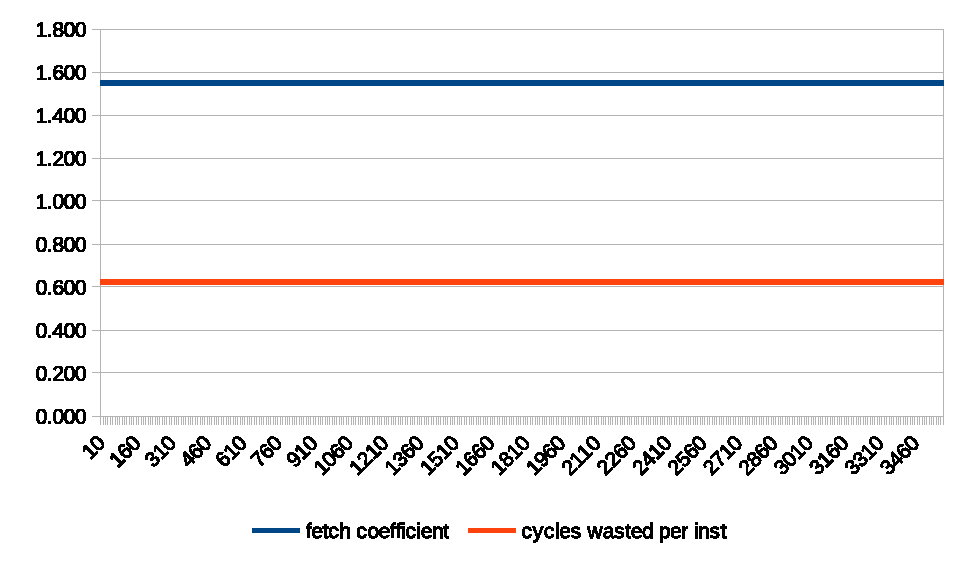
\includegraphics[width=\textwidth]{img/graph/embench/nsichneu_fetch_waste.eps}
        \caption{Fetch coefficient and cycles wasted per instruction over time (ms)}
    \end{subfigure}
    \caption{Performance over time: \texttt{nsichneu}}
\end{figure}

% picojpeg   
\begin{figure}
    \begin{subfigure}{0.45\textwidth}
        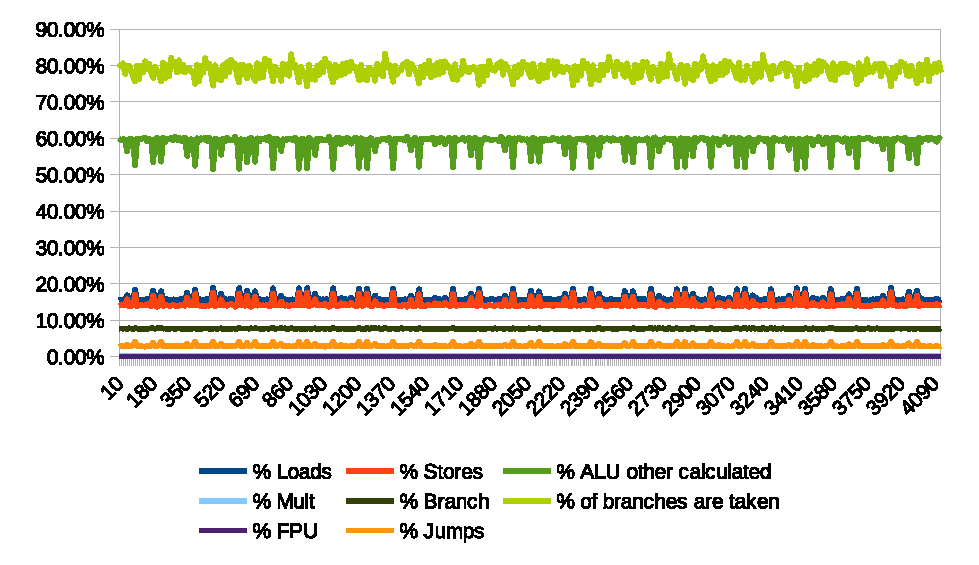
\includegraphics[width=\textwidth]{img/graph/embench/picojpeg_inst.eps}
        \caption{Instruction behavior over time (ms)}
    \end{subfigure}
    \begin{subfigure}{0.45\textwidth}
        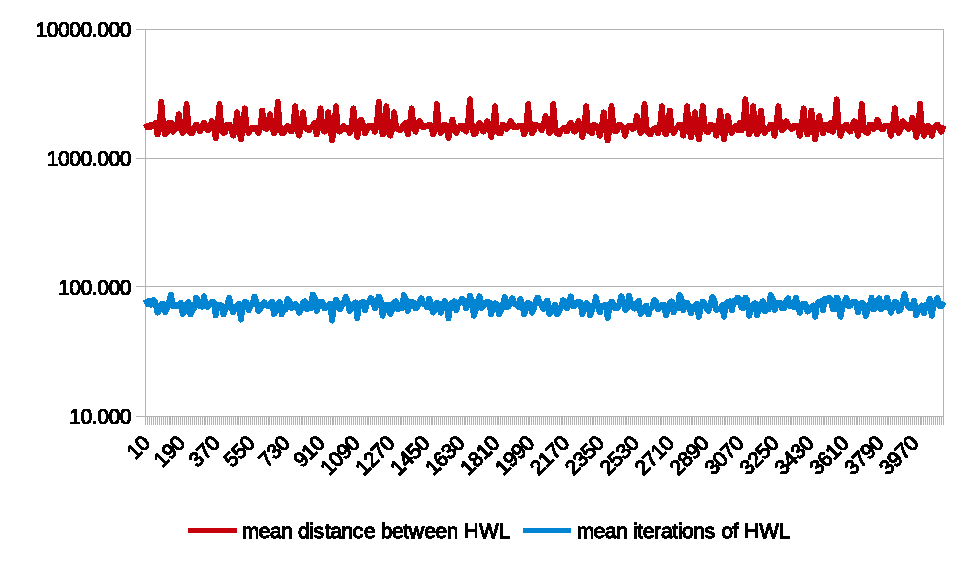
\includegraphics[width=\textwidth]{img/graph/embench/picojpeg_hwl.eps}
        \caption{\ac{HWL} behavior over time (ms)}
    \end{subfigure}
    \begin{subfigure}{0.45\textwidth}
        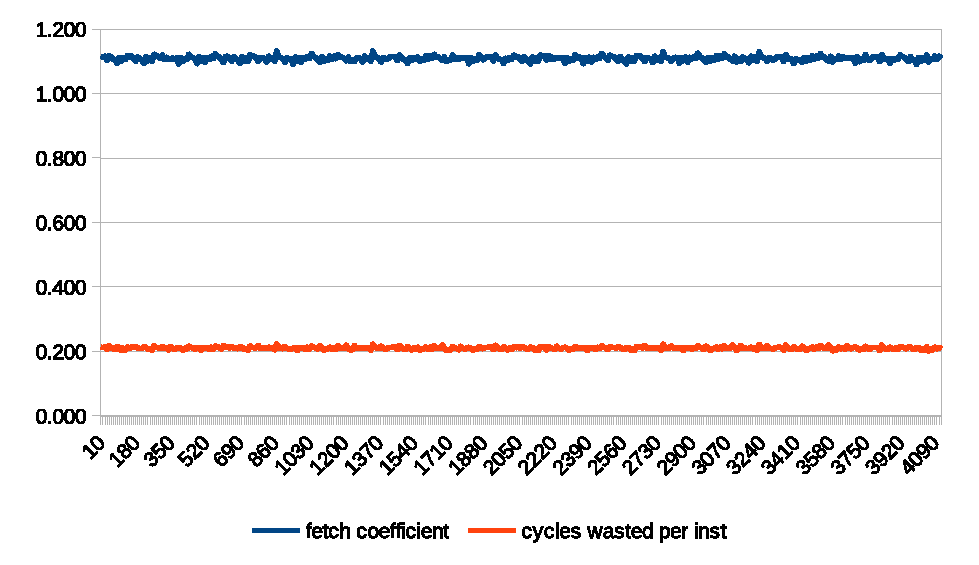
\includegraphics[width=\textwidth]{img/graph/embench/picojpeg_fetch_waste.eps}
        \caption{Fetch coefficient and cycles wasted per instruction over time (ms)}
    \end{subfigure}
    \caption{Performance over time: \texttt{picojpeg}}
\end{figure}

% qrduino   
\begin{figure}
    \begin{subfigure}{0.45\textwidth}
        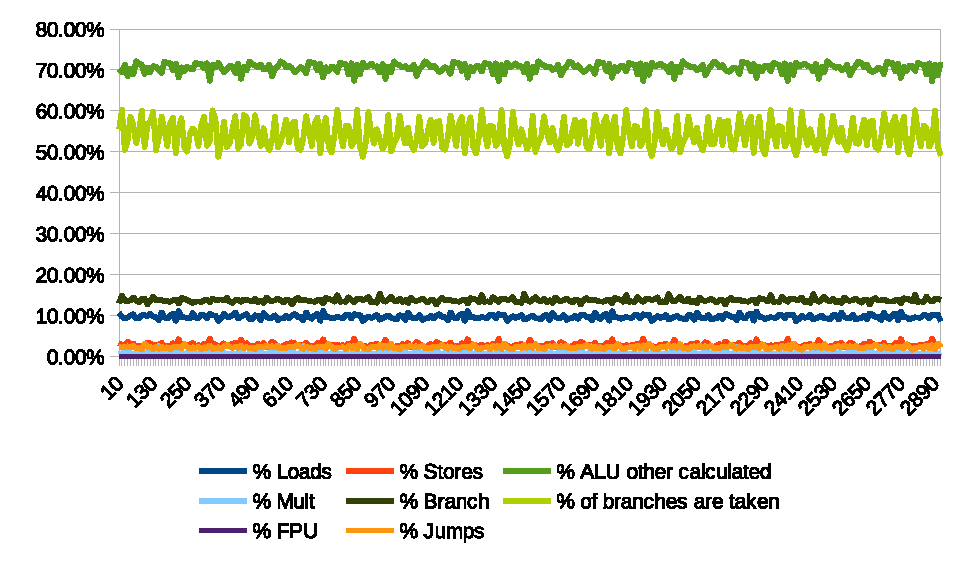
\includegraphics[width=\textwidth]{img/graph/embench/qrduino_inst.eps}
        \caption{Instruction behavior over time (ms)}
    \end{subfigure}
    \begin{subfigure}{0.45\textwidth}
        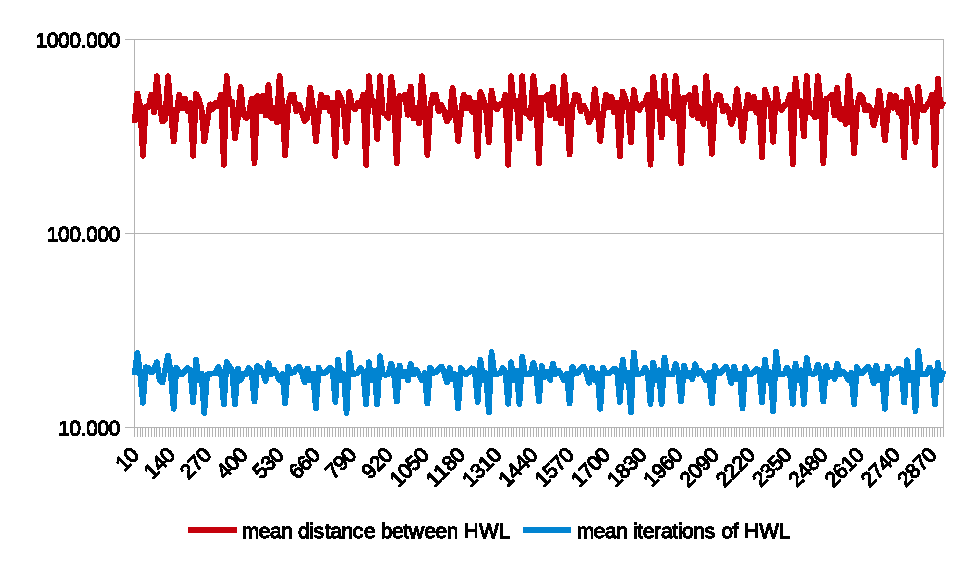
\includegraphics[width=\textwidth]{img/graph/embench/qrduino_hwl.eps}
        \caption{\ac{HWL} behavior over time (ms)}
    \end{subfigure}
    \begin{subfigure}{0.45\textwidth}
        \includegraphics[width=\textwidth]{img/graph/embench/qrduino_fetch_waste.eps}
        \caption{Fetch coefficient and cycles wasted per instruction over time (ms)}
    \end{subfigure}
    \caption{Performance over time: \texttt{qrduino}}
\end{figure}

% sglib-combined   
\begin{figure}
    \begin{subfigure}{0.45\textwidth}
        \includegraphics[width=\textwidth]{img/graph/embench/sglib-combined_inst.eps}
        \caption{Instruction behavior over time (ms)}
    \end{subfigure}
    \begin{subfigure}{0.45\textwidth}
        \includegraphics[width=\textwidth]{img/graph/embench/sglib-combined_hwl.eps}
        \caption{\ac{HWL} behavior over time (ms)}
    \end{subfigure}
    \begin{subfigure}{0.45\textwidth}
        \includegraphics[width=\textwidth]{img/graph/embench/sglib-combined_fetch_waste.eps}
        \caption{Fetch coefficient and cycles wasted per instruction over time (ms)}
    \end{subfigure}
    \caption{Performance over time: \texttt{sglib-combined}}
\end{figure}

% slre   
\begin{figure}
    \begin{subfigure}{0.45\textwidth}
        \includegraphics[width=\textwidth]{img/graph/embench/slre_inst.eps}
        \caption{Instruction behavior over time (ms)}
    \end{subfigure}
    \begin{subfigure}{0.45\textwidth}
        \includegraphics[width=\textwidth]{img/graph/embench/slre_hwl.eps}
        \caption{\ac{HWL} behavior over time (ms)}
    \end{subfigure}
    \begin{subfigure}{0.45\textwidth}
        \includegraphics[width=\textwidth]{img/graph/embench/slre_fetch_waste.eps}
        \caption{Fetch coefficient and cycles wasted per instruction over time (ms)}
    \end{subfigure}
    \caption{Performance over time: \texttt{slre}}
\end{figure}

% st   
\begin{figure}
    \begin{subfigure}{0.45\textwidth}
        \includegraphics[width=\textwidth]{img/graph/embench/st_inst.eps}
        \caption{Instruction behavior over time (ms)}
    \end{subfigure}
    \begin{subfigure}{0.45\textwidth}
        \includegraphics[width=\textwidth]{img/graph/embench/st_hwl.eps}
        \caption{\ac{HWL} behavior over time (ms)}
    \end{subfigure}
    \begin{subfigure}{0.45\textwidth}
        \includegraphics[width=\textwidth]{img/graph/embench/st_fetch_waste.eps}
        \caption{Fetch coefficient and cycles wasted per instruction over time (ms)}
    \end{subfigure}
    \caption{Performance over time: \texttt{st}}
\end{figure}

% statemate   
\begin{figure}
    \begin{subfigure}{0.45\textwidth}
        \includegraphics[width=\textwidth]{img/graph/embench/statemate_inst.eps}
        \caption{Instruction behavior over time (ms)}
    \end{subfigure}
    \begin{subfigure}{0.45\textwidth}
        \includegraphics[width=\textwidth]{img/graph/embench/statemate_fetch_waste.eps}
        \caption{Fetch coefficient and cycles wasted per instruction over time (ms)}
    \end{subfigure}
    \caption{Performance over time: \texttt{statemate}}
\end{figure}

% ud   
\begin{figure}
    \begin{subfigure}{0.45\textwidth}
        \includegraphics[width=\textwidth]{img/graph/embench/ud_inst.eps}
        \caption{Instruction behavior over time (ms)}
    \end{subfigure}
    \begin{subfigure}{0.45\textwidth}
        \includegraphics[width=\textwidth]{img/graph/embench/ud_hwl.eps}
        \caption{\ac{HWL} behavior over time (ms)}
    \end{subfigure}
    \begin{subfigure}{0.45\textwidth}
        \includegraphics[width=\textwidth]{img/graph/embench/ud_fetch_waste.eps}
        \caption{Fetch coefficient and cycles wasted per instruction over time (ms)}
    \end{subfigure}
    \caption{Performance over time: \texttt{ud}}
\end{figure}

% wikisort   
\begin{figure}
    \begin{subfigure}{0.45\textwidth}
        \includegraphics[width=\textwidth]{img/graph/embench/wikisort_inst.eps}
        \caption{Instruction behavior over time (ms)}
    \end{subfigure}
    \begin{subfigure}{0.45\textwidth}
        \includegraphics[width=\textwidth]{img/graph/embench/wikisort_hwl.eps}
        \caption{\ac{HWL} behavior over time (ms)}
    \end{subfigure}
    \begin{subfigure}{0.45\textwidth}
        \includegraphics[width=\textwidth]{img/graph/embench/wikisort_fetch_waste.eps}
        \caption{Fetch coefficient and cycles wasted per instruction over time (ms)}
    \end{subfigure}
    \caption{Performance over time: \texttt{wikisort}}
\end{figure}

\FloatBarrier
\section{Other}
% dhrystone   
\begin{figure}
    \begin{subfigure}{0.45\textwidth}
        \includegraphics[width=\textwidth]{img/graph/riscv/dhrystone_inst.eps}
        \caption{Instruction behavior over time (ms)}
    \end{subfigure}
    \begin{subfigure}{0.45\textwidth}
        \includegraphics[width=\textwidth]{img/graph/riscv/dhrystone_fetch_waste.eps}
        \caption{Fetch coefficient and cycles wasted per instruction over time (ms)}
    \end{subfigure}
    \caption{Performance over time: Dhrystone}
\end{figure}

% Coremark   
\begin{figure}
    \begin{subfigure}{0.45\textwidth}
        \includegraphics[width=\textwidth]{img/graph/coremark/coremark_inst.eps}
        \caption{Instruction behavior over time (ms)}
    \end{subfigure}
    \begin{subfigure}{0.45\textwidth}
        \includegraphics[width=\textwidth]{img/graph/coremark/coremark_hwl.eps}
        \caption{\ac{HWL} behavior over time (ms)}
    \end{subfigure}
    \begin{subfigure}{0.45\textwidth}
        \includegraphics[width=\textwidth]{img/graph/coremark/coremark_fetch_waste.eps}
        \caption{Fetch coefficient and cycles wasted per instruction over time (ms)}
    \end{subfigure}
    \caption{Performance over time: Coremark}
\end{figure}

% Render bibliograhy and acronyms if rendered standalone
\isstandalone
\bibliographystyle{IEEEtran}
\bibliography{bibliography}
\subfile{abbreviations.tex}
\fi

\end{document} 
